
\section{Prior considerations}


\subsection{Data transformations}

As can be observed in Table \ref{table:general_statistics}, the units of our data points are on different scales. As discussed in \cite{muller2016introduction} it is not recommended for optimization procedures as machine learning estimations to work with such data directly, as a consequence  
all the work developed in this document uses Equation \ref{eq:1_4} to scale the data points.


\begin{equation}
sc(x_{i}) = \frac{x_{i}-x_{min}}{x_{max}-x_{min}}
\label{eq:1_4}
\end{equation}

It is commented in \cite{makridakis2008forecasting} that abrupt changes in time series can increase the modeling difficulties due to properties of the respective derivates, as can be seen in Figure \ref{fig:introduction_1} $y_{t}$ explodes near the end of 2017, we, therefore, implemented the natural logarithm transformation to smooth the rate of change of $y_{t}$.

\begin{equation}
f (y_{t}) = ln(y_{t})
\label{eq:1_5}
\end{equation}

\subsection{Data Interpolation}
Using the \textbf{Deepblue bot} depends on the servers of Google and Twitter replying to the request; therefore, we do not have continuous data for some days. To overcome this difficulty, a third-degree polynomial was fitted between the missing days to fill up the gaps for the year 2018. The full mathematical description of cubic interpolation over one dimension can be found in \cite{chapra1998numerical}, no further optimization or performance metric was calculated to asses the adequateness of the interpolation\footnote{ For the year 2018 we have 321 days for analysis, only 13 days needed interpolation}. For the year 2019, the data does not have gaps from April to May; however, there is no data available from January to March.


\subsection{The Naive Forecast}

The naive forecast ($\hat{y}_{t+1}=y_{t}$) as explained in \cite{makridakis2008forecasting} is one of the simplest models and is typically used as the baseline for assessing the performance of more complicated models.


\subsection{Cross-Validation for Time Series: Rolling Forecasting Origin}

Using cross-validation on time series is different from other regression problems because there exists a temporal dependency between data points $x_{i}$. In \cite{hyndman2006another} the concept of \textbf{rolling forecasting origin} is explained as follows:

\begin{enumerate}
	\item \textit{ Select the observation at time $t + i$ where for the test set, and use the observations at times $1, 2, . . . , t+i-1$ to estimate the forecasting model. Compute the error on the forecast for time $t + 1$.}
	\item \textit{ Repeat the above step for$1, 2, . . . , N-t$ where $N$ is the total number of observations.} From here on, the number of test value is defined as $N-t=CV_{Rol}$.
	\item \textit{ Compute the forecast accuracy measures based on the errors obtained.}
\end{enumerate}

\begin{figure}[htpb!] % Defines figure environment
	\centering % Centers your figure
	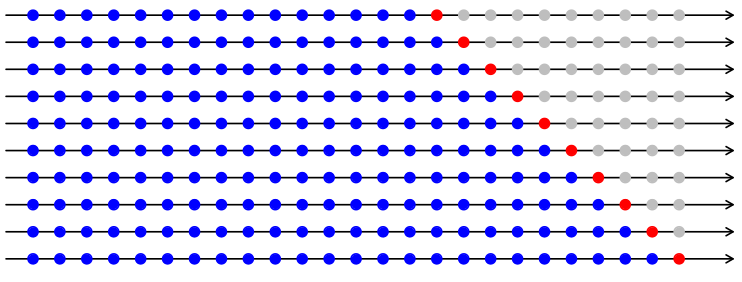
\includegraphics[width=0.4\textwidth]{notebooks/data/cv_time.png} % Includes your figure and defines %the size
	\caption{\textit{ Rolling forecasting origin scheme. One-step forecasts. The blue points are training sets,the red points are test sets and the grey points are ignored.} (taken from \cite{hyndman2006another} )} % For your caption
	\label{fig:cross validation} % If you want to label your figure for in-text references
\end{figure}



\section{Time Series Analysis using Classical Decompositional model}

Here we explore the possibility of predicting the next day average price by only using values of the past. Formally this is known as a one-time step forecast
by autoregression models. As explained in \cite{makridakis2008forecasting} the classical Decompositional approach states that the Equation \ref{eq:4_1} holds.  

\begin{equation}
y_{t}=S_{t}+T_{t}+E_{t}
\label{eq:4_1}
\end{equation}

Where $S,T,E$ stand for \textit{Seasonal}, \textit{Trend} and \textit{Error}. To estimate $T$ we explored two methods, namely \emph{odd moving averages} and \emph{simple exponential smoothing}. \emph{odd moving averages} is governed by Equation \ref{eq:4_2}, where $y_{t}$ is the price at time-step $t \in \mathbb{N}$, $odd \in \mathbb{N}$ the parameter of the steps averages and $N$ the maximum index of the series which can be regarded as the present. In equation \ref{eq:4_2}, the limits of the summation must be approximated to the smallest integer.


\begin{equation}
T^{mv}_{t}(odd)=\begin{cases}
\sum_{i=y_{t}-odd/2}^{y_{t}+odd/2} \frac{y_{i} }{odd} , & \text{if $t<odd$}.\\
\sum_{i=y_{t}-odd/2}^{N} \frac{y_{i} }{odd}, & \text{otherwise}.
\end{cases}
\label{eq:4_2}
\end{equation}

\emph{simple exponential smoothing} is governed by in Equation \ref{eq:SES} Where $\beta \in [0,1]$ is the smoothing parameter.


\begin{equation}
T^{ses}_{t}(\beta)=\begin{cases}
y_{0}  , & \text{if $t=0$}.\\
\beta y_{t}+(1-\beta)T^{ses}_{t-1}, & \text{otherwise}.
\end{cases}
\label{eq:SES}
\end{equation}

For the following section, we will refer by the trend calculated with moving averages and simple exponential smoothing only by $T^{mv}$ and $T^{ses}$ respectively.


\subsection{Decomposition, Moving Averages based}


In Figure \ref{fig:mv_2016_2019} we can see moving averages $odd \in [87,150,297]$. Let us select $odd=150$ moving average as $T^{mv}$. 

\begin{figure}[!htb]
	\center{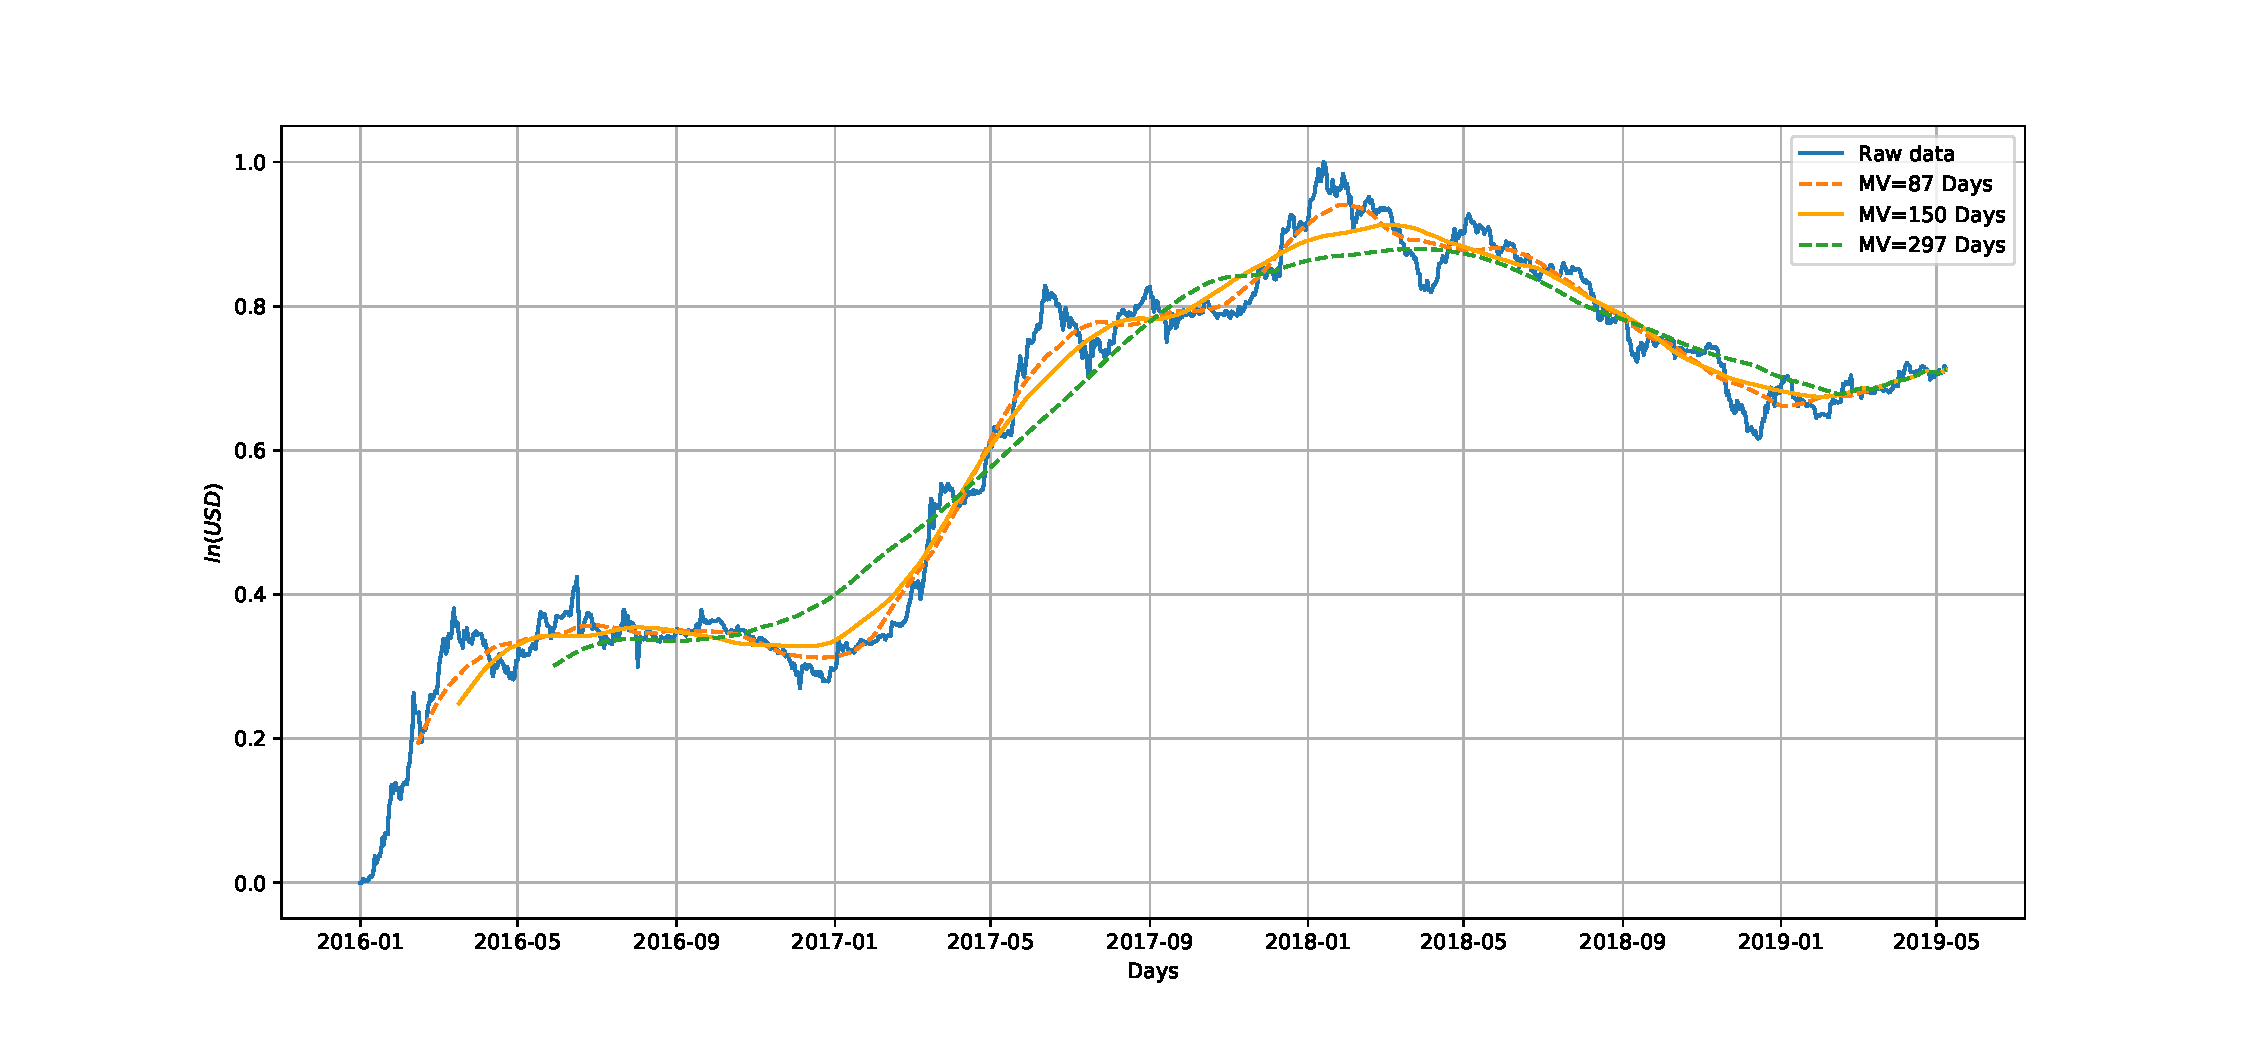
\includegraphics[width=\textwidth]
		{notebooks/data/movingAverages.pdf}}
	\caption{\label{fig:mv_2016_2019}  moving averages exploration}
\end{figure}

By subtracting $y$ and $T^{mv}$ we obtain the combination $S+E$, we call this subtraction the \textit{de-trended} series. We now assume that the \textit{seasonal} component is repeated over the years per month. We also assumed that the error component has a normal distribution \footnote{by the central limit theorem} with $\mu=0$, as a result, by averaging the de-trended time series per month over the years we get an estimate of the \textit{seasonal} average per month. In it is mentioned in \cite{makridakis2008forecasting} that this 12 element set is known as the \textit{seasonal indexes}.


\begin{figure}[!tbp]
	\centering
	\begin{minipage}[b]{0.49\textwidth}
		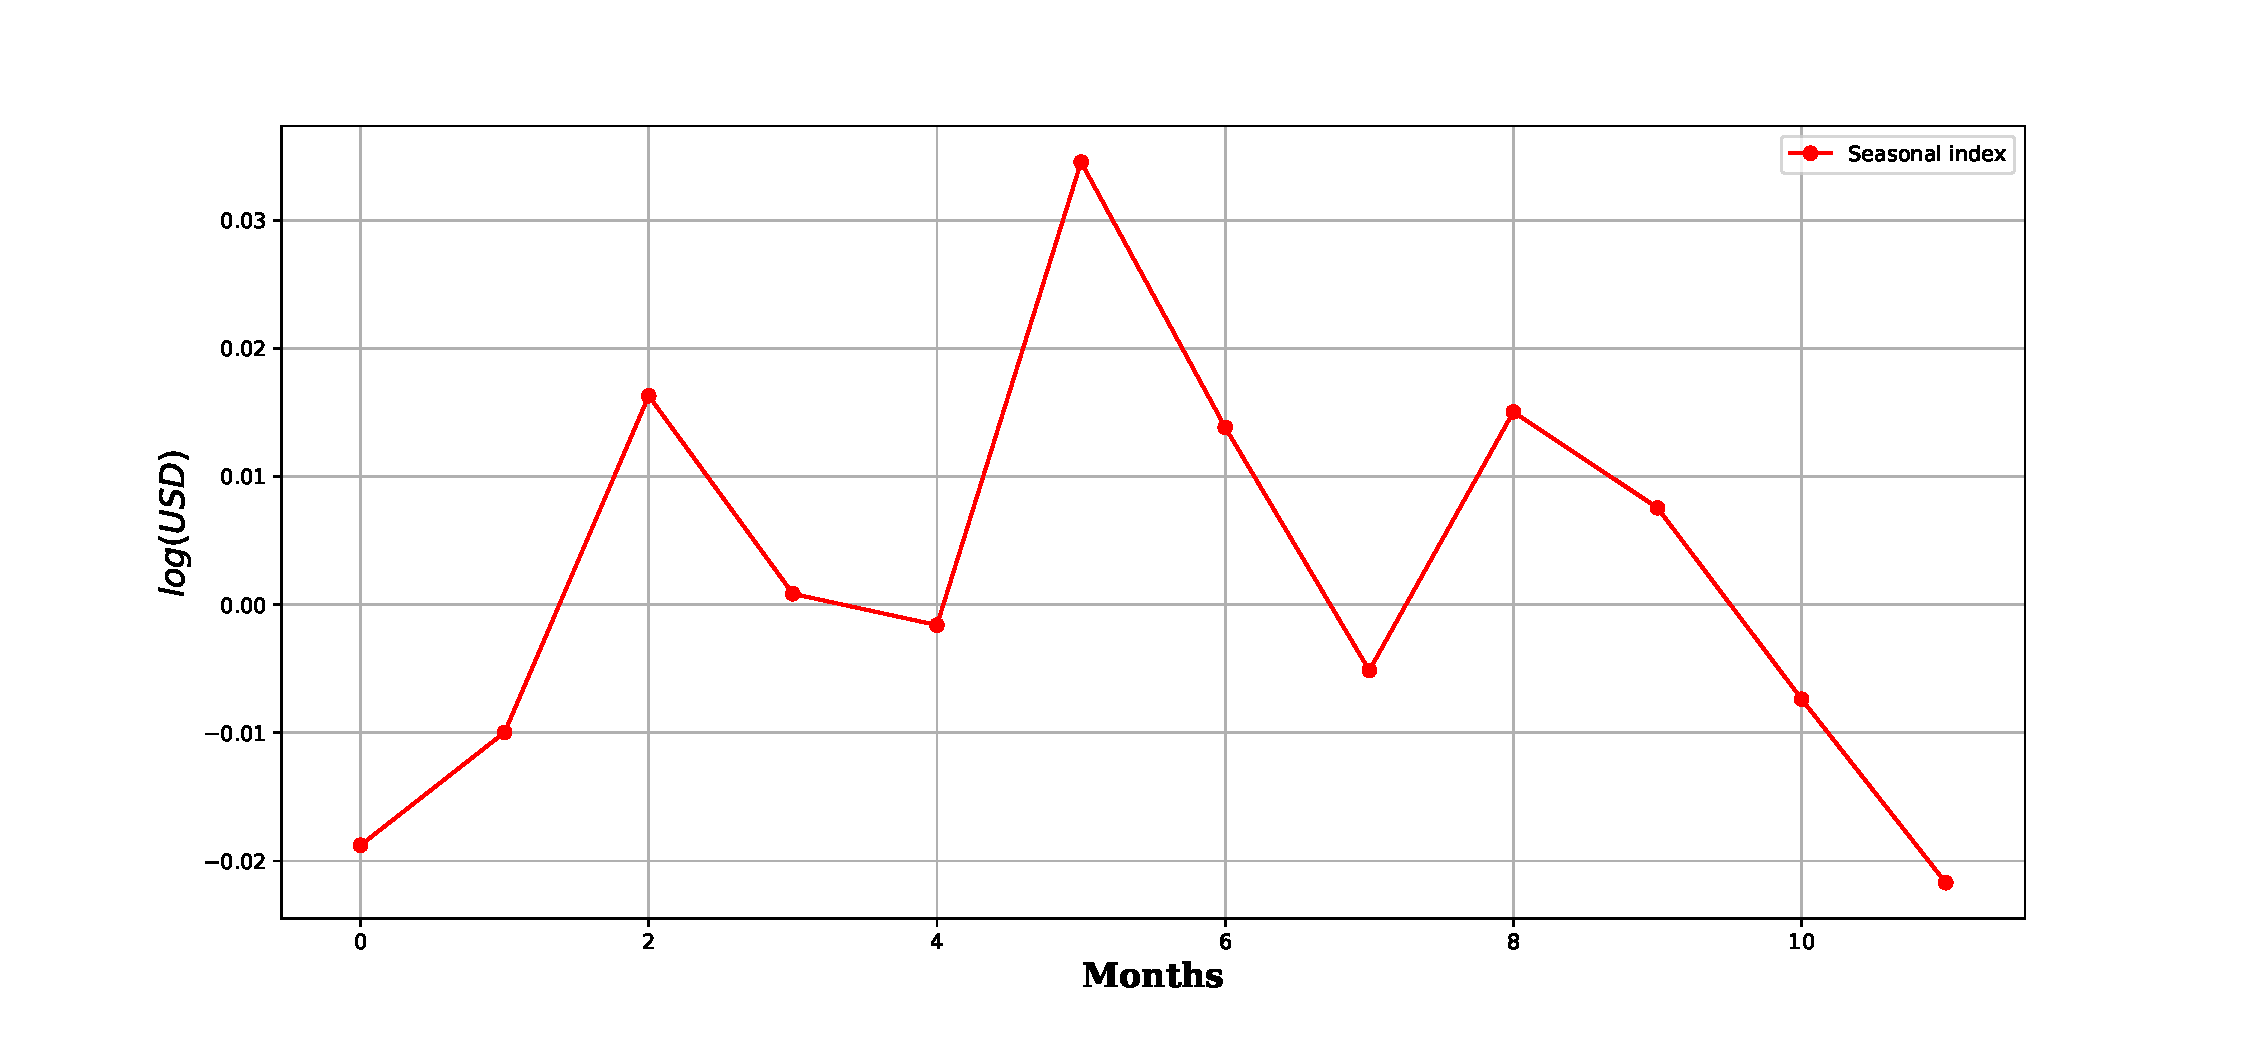
\includegraphics[width=\textwidth]{notebooks/data/seasonal_index.pdf}
		\caption{Seasonal indices.}
	\end{minipage}
	\hfill
	\begin{minipage}[b]{0.49\textwidth}
		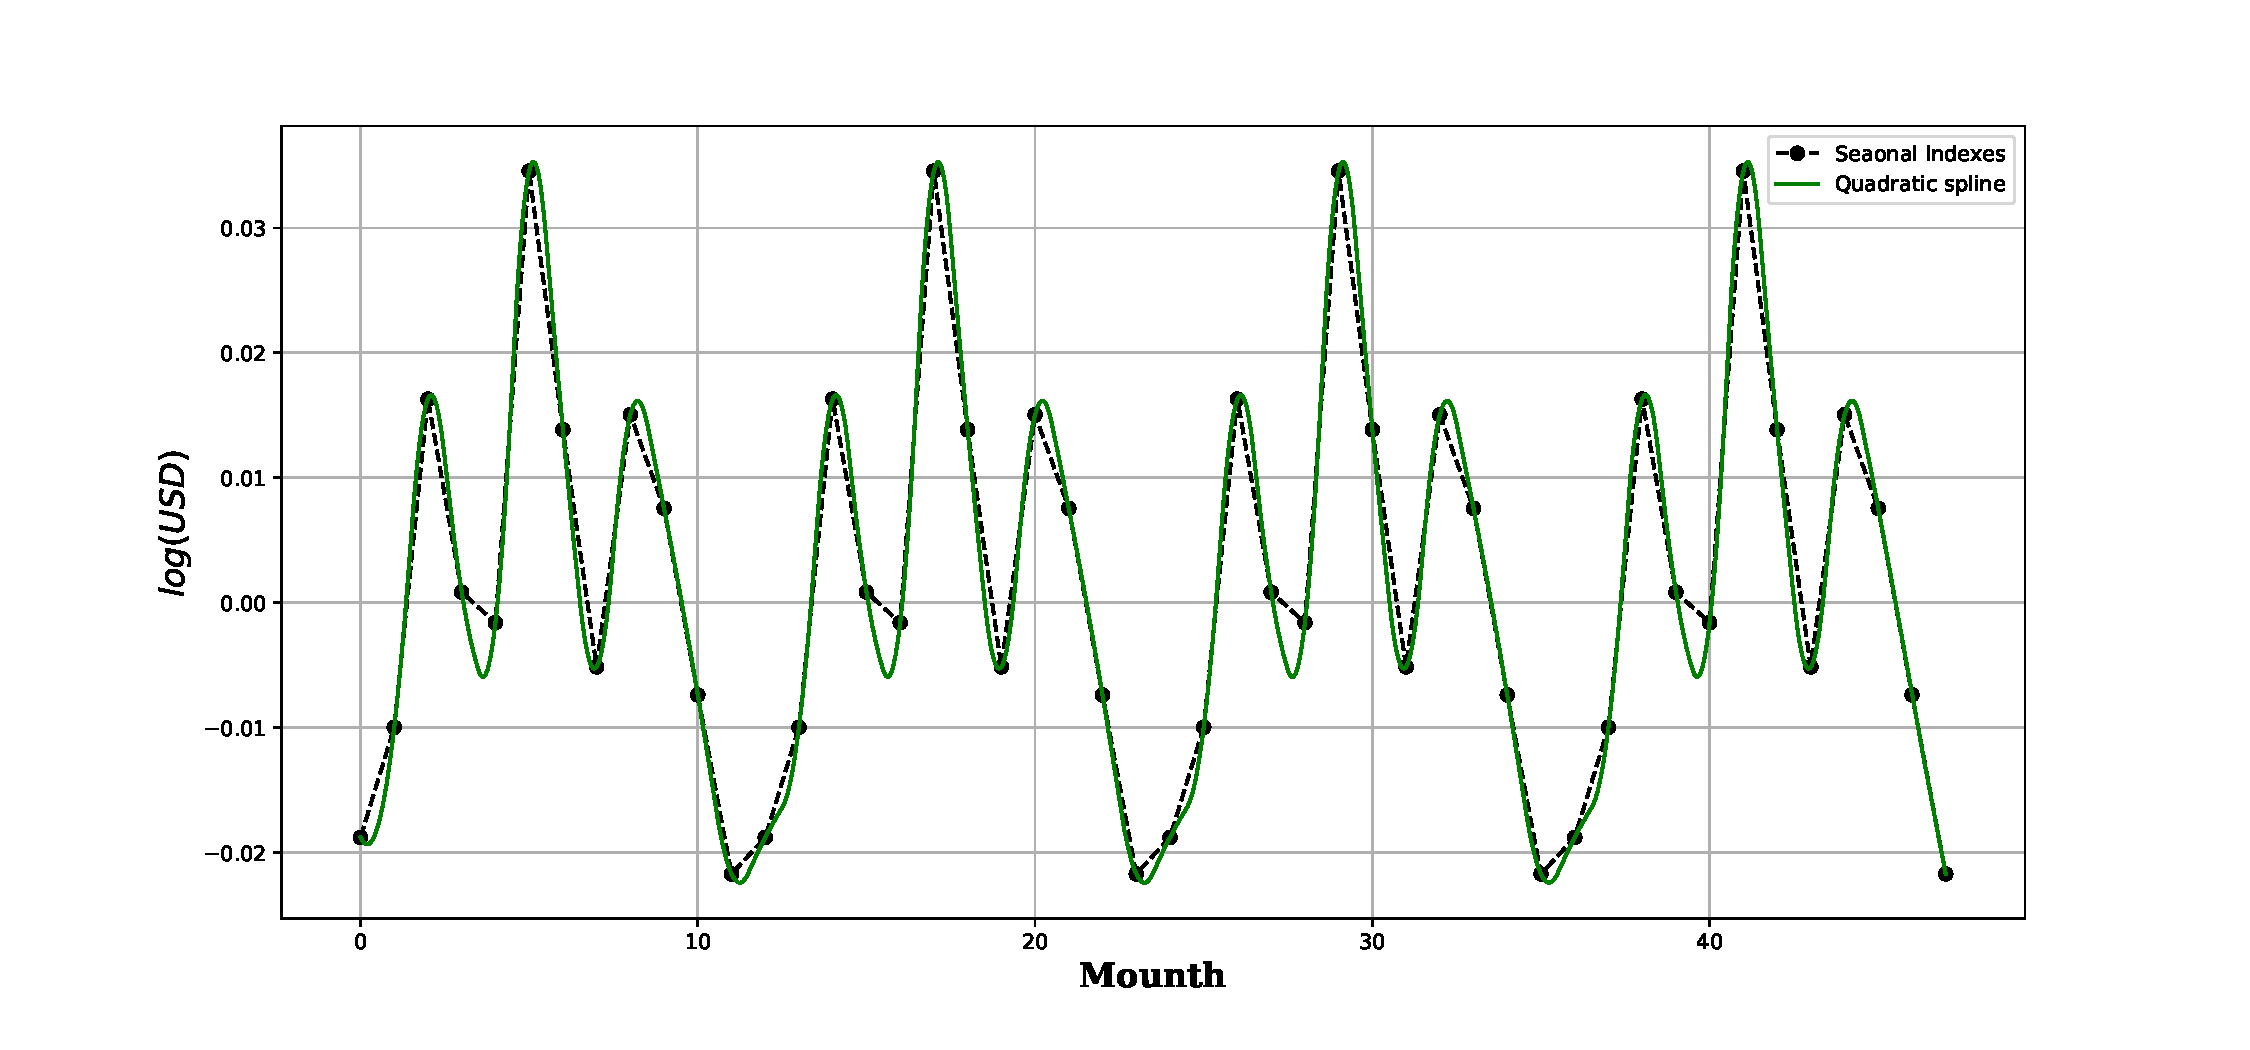
\includegraphics[width=\textwidth]{notebooks/data/seasonal_interpolation.pdf}
		\caption{Seasonal interpolation.}
		\label{fig:seasonal_interpolation}
	\end{minipage}
\end{figure}


We decided to perform a 2-tail t-statistics test between $y=T^{mv}+S$ and $y'=T^{mv}$ to evaluate the null hypothesis $H_{0}$ that the difference between $y$ and $y'$ is produced by chance only, rendering $S$ just like noise.



\begin{table}[h!]
	\begin{center}
		\begin{tabular}{||c c c||} 
			\hline
			RV & t-value & p-value \\ [0.5ex] 
			\hline\hline
			$y$,$y'$ & 0.27 & 0.78  \\ 
			\hline
		\end{tabular}
		\caption{T-test for Seasonality.}
		\label{table:t_test}
	\end{center}
\end{table}

As can be observed in table \ref{table:t_test} the $p-value$ is near one, which tell us not to reject $H_{0}$. Following this conclusion we modified  \ref{eq:4_1} to \ref{eq:4_3} 

\begin{equation}
y_{t}=T^{mv}_{t}+E_{t}
\label{eq:4_3}
\end{equation}

Finally, we obtain the $E$ by calculating the relationship  $E=y-T^{mv}$. Figure \ref{fig:error} shows $E$. 

\begin{figure}[htpb!] % Defines figure environment
	\centering % Centers your figure
	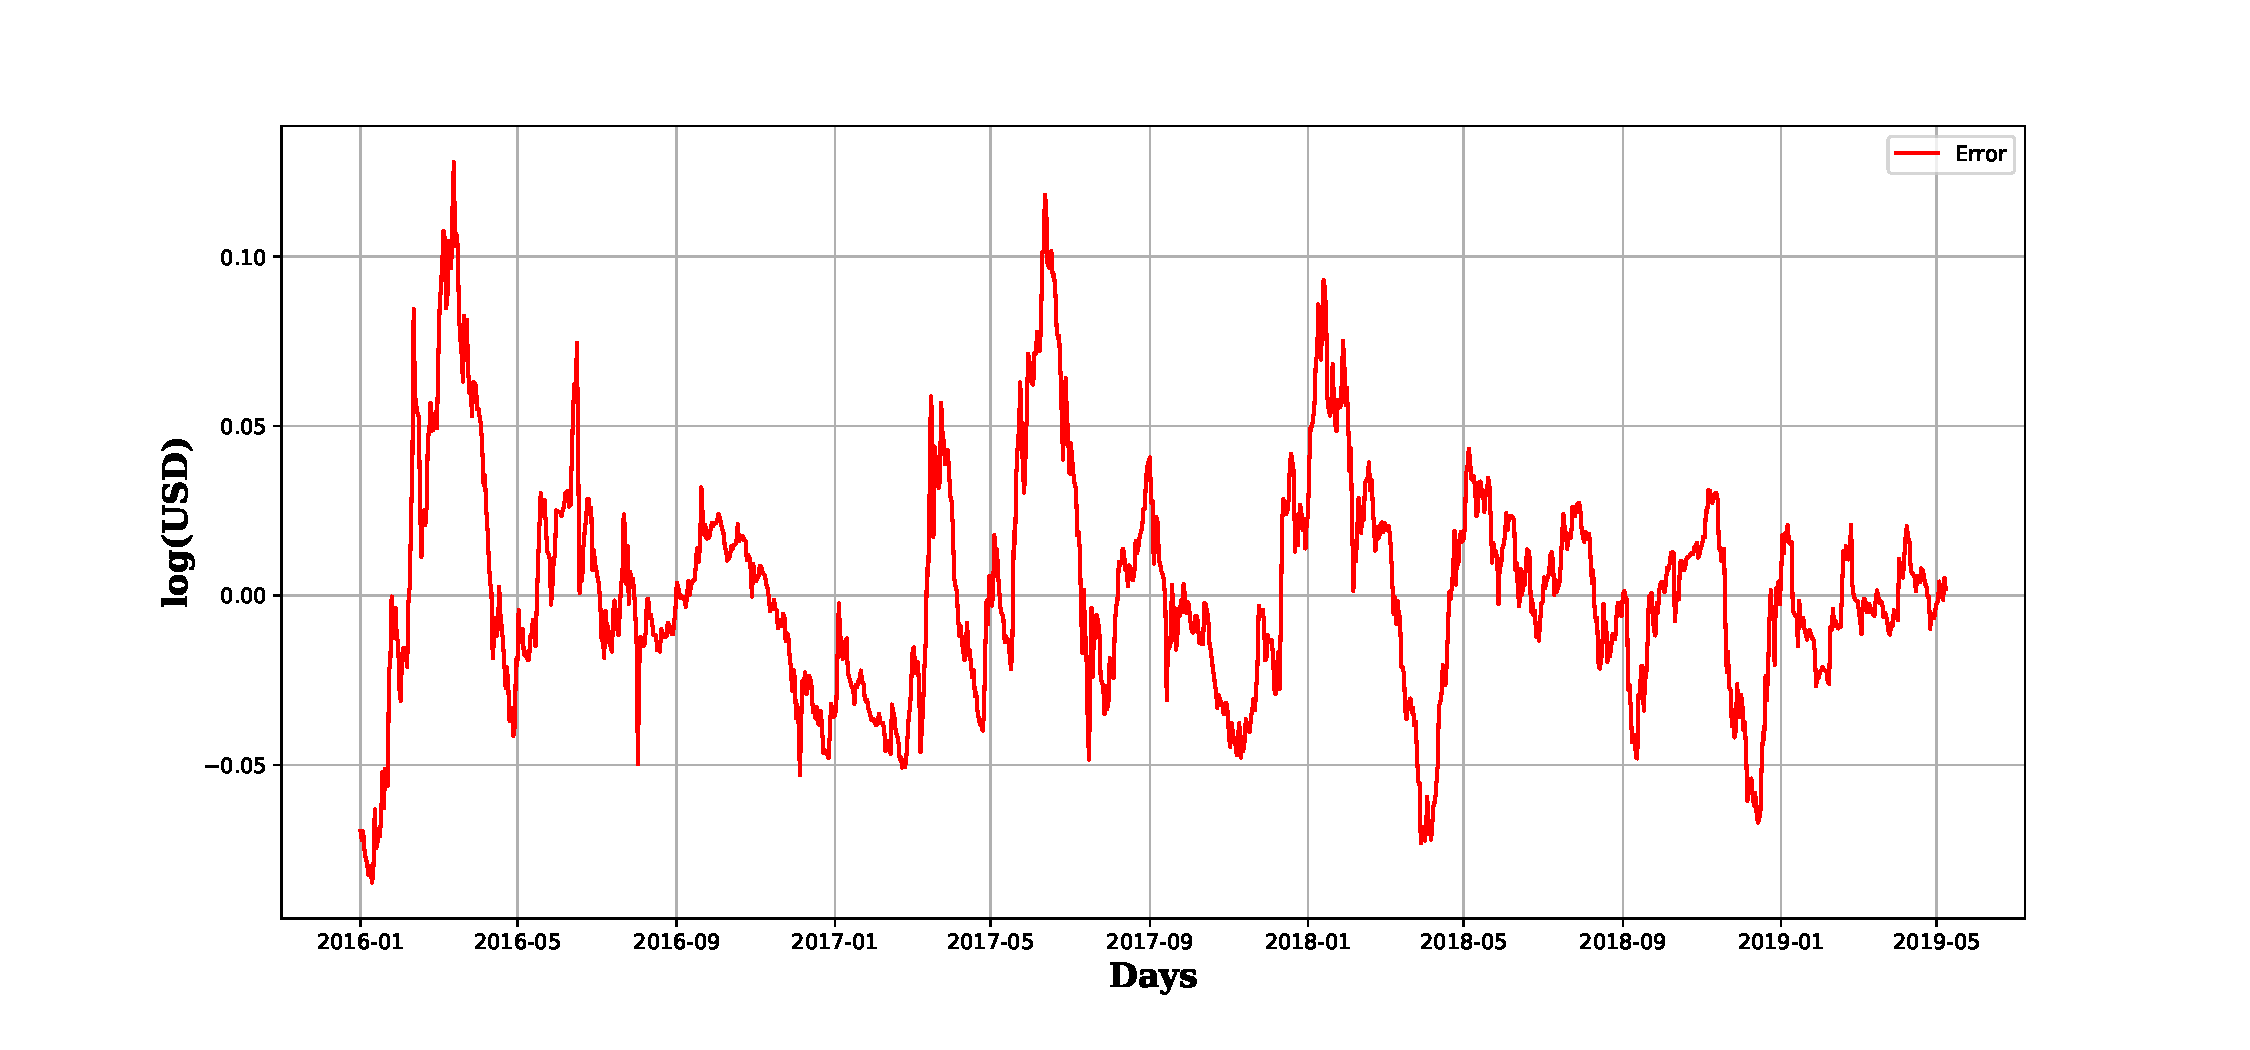
\includegraphics[width=\textwidth]{notebooks/data/Residual_error_u.pdf} % Includes your figure and defines %the size
	\caption{Error plot. $E$} % For your caption
	\label{fig:error} % If you want to label your figure for in-text references
\end{figure}

In figure \ref{fig:single_plot} we can observe the full decomposition based on moving averages.

\begin{figure}[htpb!] % Defines figure environment
	\centering % Centers your figure
	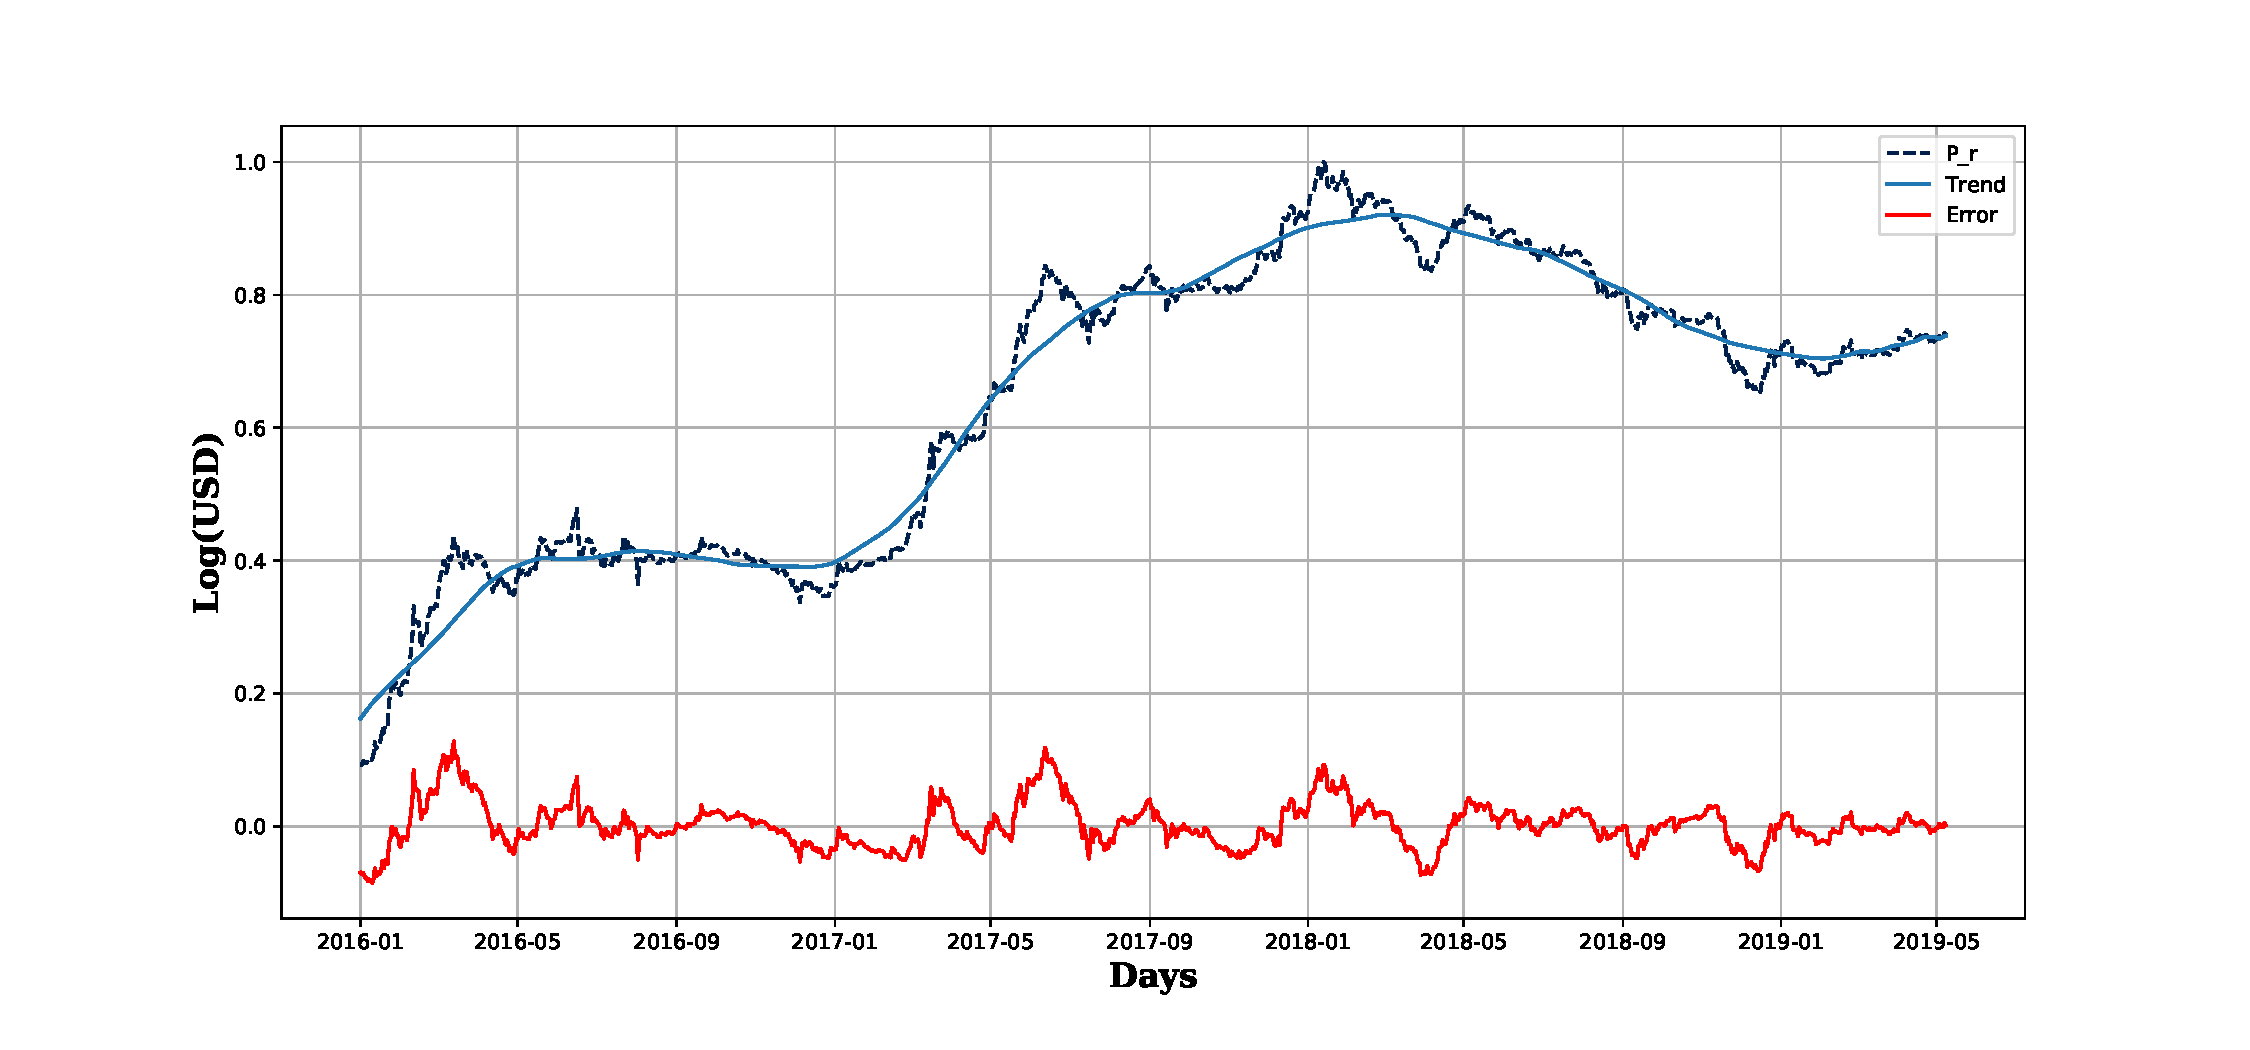
\includegraphics[width=\textwidth]{notebooks/data/single_plot.pdf} % Includes your figure and defines %the size
	\caption{Single plot decomposition moving averages based.} % For your caption
	\label{fig:single_plot} % If you want to label your figure for in-text references
\end{figure}


\subsubsection{Ridge Regression for $T^{mv}$ and $E$}


In this section we try to model the component $T^{mv}$ and $E$ of Equation \ref{eq:4_3} using the decision functions $\mathcal{D}$ based on \emph{Ridge regression} \footnote{Implemented using \cite{scikitlearn22}}.\\

Ridge regression is a supervised learning algorithm that minimized the quadric loss to fit a linear relationship between the features vector and the target variable. Using single value decomposition, the minimum quadric loss parameters can be encoded in a $W'_{opt} \in \mathbb{R}^{m \times 1}$ matrix, where $m$ is the number of features. In Equation \ref{eq:4_4} $\Phi$ is a matrix of $\mathbb{R}^{N \times m}$ where $N$ is the number of data points. $Z$ is a column vector $\mathbb{R}^{N}$ containing the target variable. $\alpha \in {\rm I\!R^{>0}}$ is a penalization factor over the fitted parameters to control the variance of the model.\\


\begin{equation}
W_{opt}'=(\Phi'\Phi+\alpha^2I)^{-1}\Phi'Z
\label{eq:4_4}
\end{equation}

Using this representation, the $m$ dimension of our matrix $\Phi$ is our main free parameter. $m$ can be regarded as the number of past time steps that we believe have a linear relationship with the $t+1$ step of our target variable. For the next section will refer to this parameter as $lag_{max}$. Note a matrix $\Phi$ with $\mathbb{R}^{N \times lag_{max}}$ will contain the sequence from $t$ to $t-lag_{max}$ target variable observations.\\ 

Let us begin by trying to find the best $lag_{max}$ parameter using Rolling forecasting origin. To do it, we set the number of test points $CV_{Rol}=100$ (please see section 2.4 for more details) and proceed to evaluate different Ridge regression(with $\alpha=0$), from less complex $lag_{max}=1$ to  a maximum of $lag_{max}=19$, the average $\%sMAPE$ per $lag_{max}$ is plotted to compare performance. The results can seem in in Figure \ref{fig:error_sc_1_lag} and \ref{fig:trend_sc_1_lag} $E$ and $T^{mv}$ respectively.\\ 


\begin{figure}[h!]
	\centering
	
	\begin{minipage}[b]{\textwidth}
		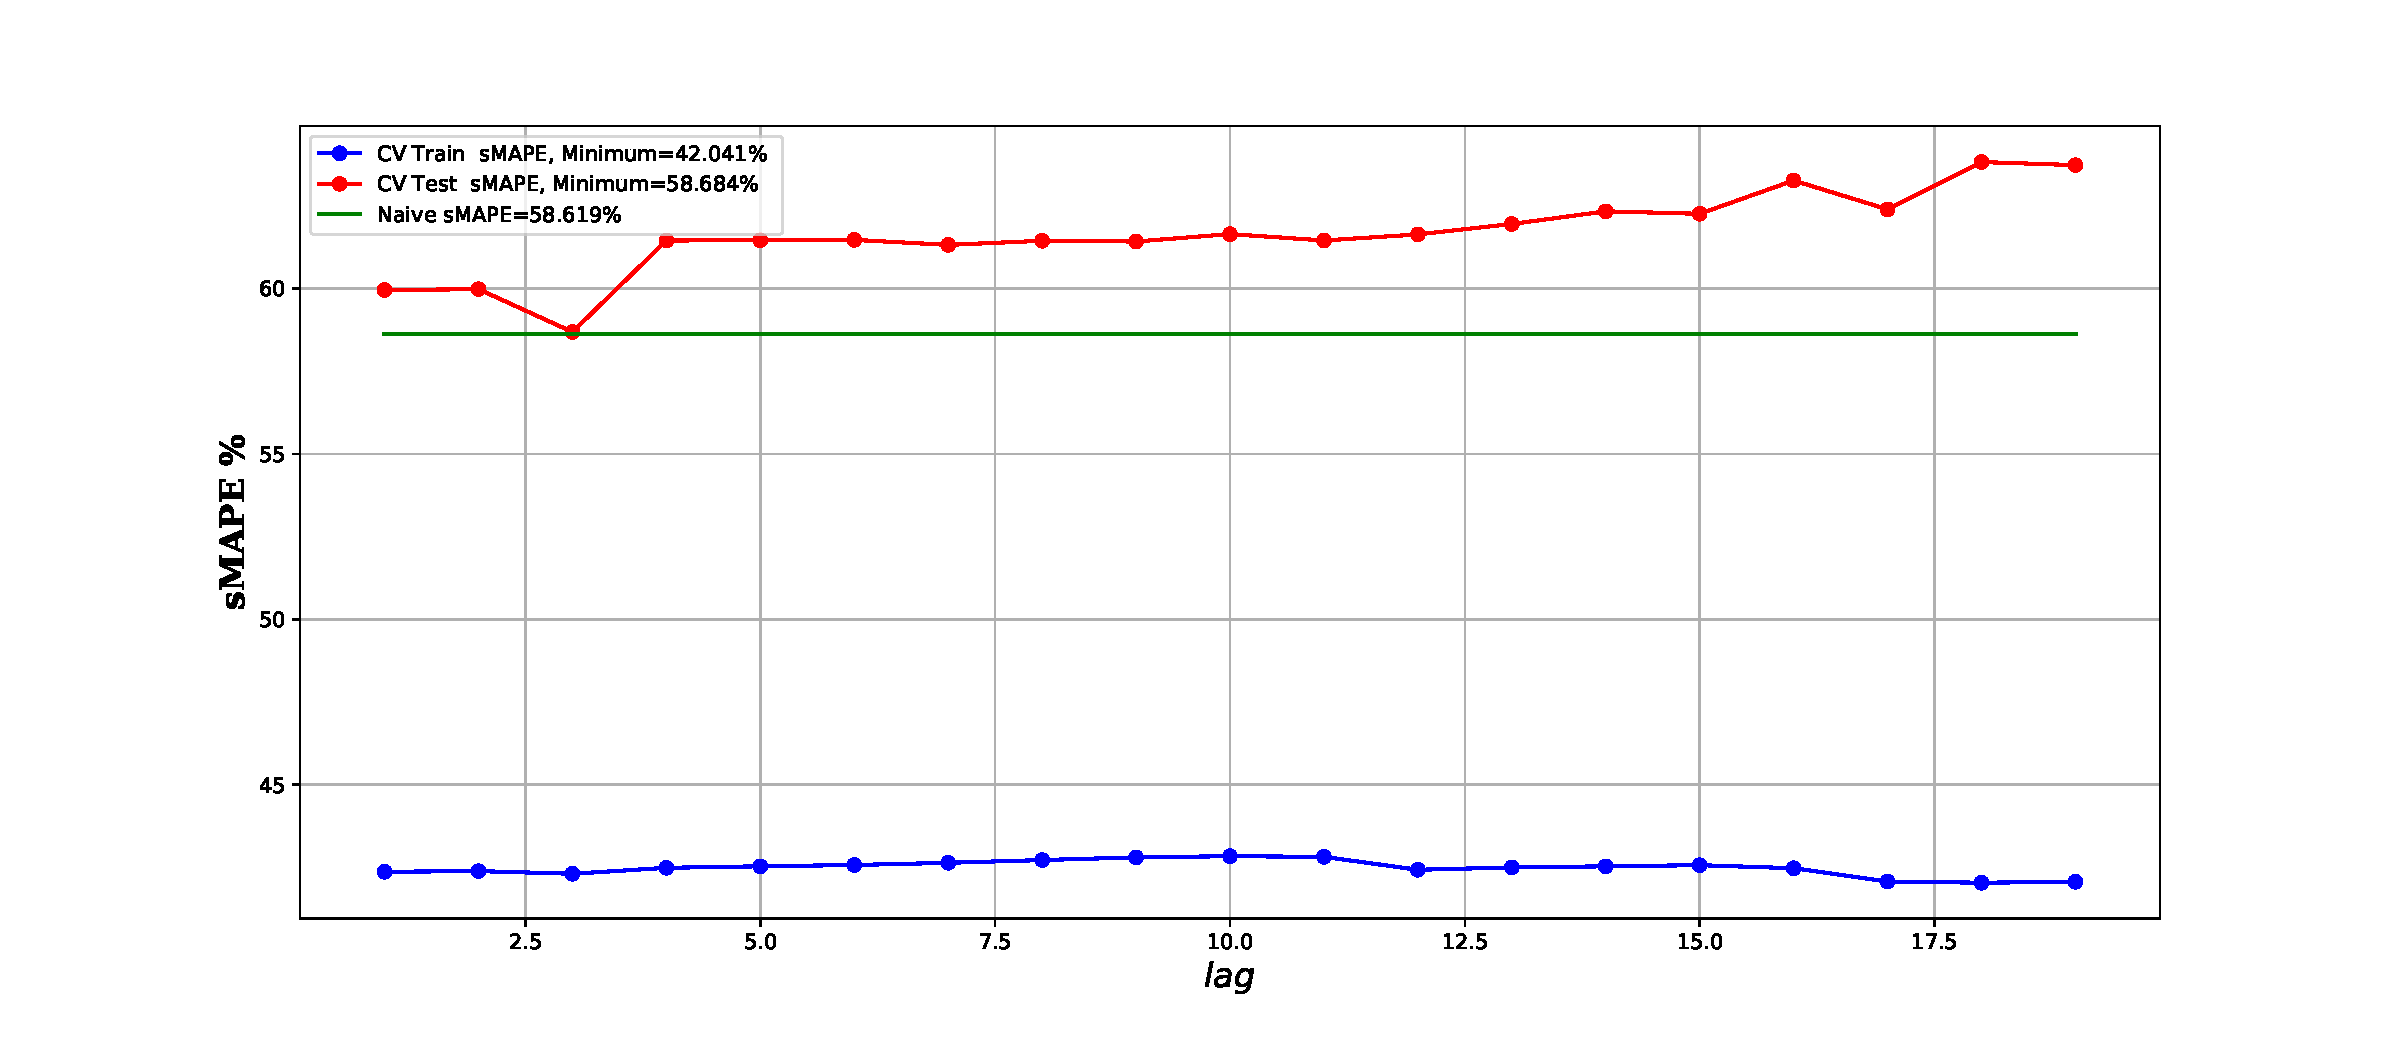
\includegraphics[width=\textwidth]{notebooks/data/error_sc_1_lag.pdf}
		\caption{\textbf{Random variable} $E$ \textbf{Model}: Ridge regression \textbf{$CV_{Rol}$}=100 \textbf{$\alpha$}=0 $lag_{max}$ }
		\label{fig:error_sc_1_lag}
	\end{minipage}
	
	\hfill
	\begin{minipage}[b]{\textwidth}
		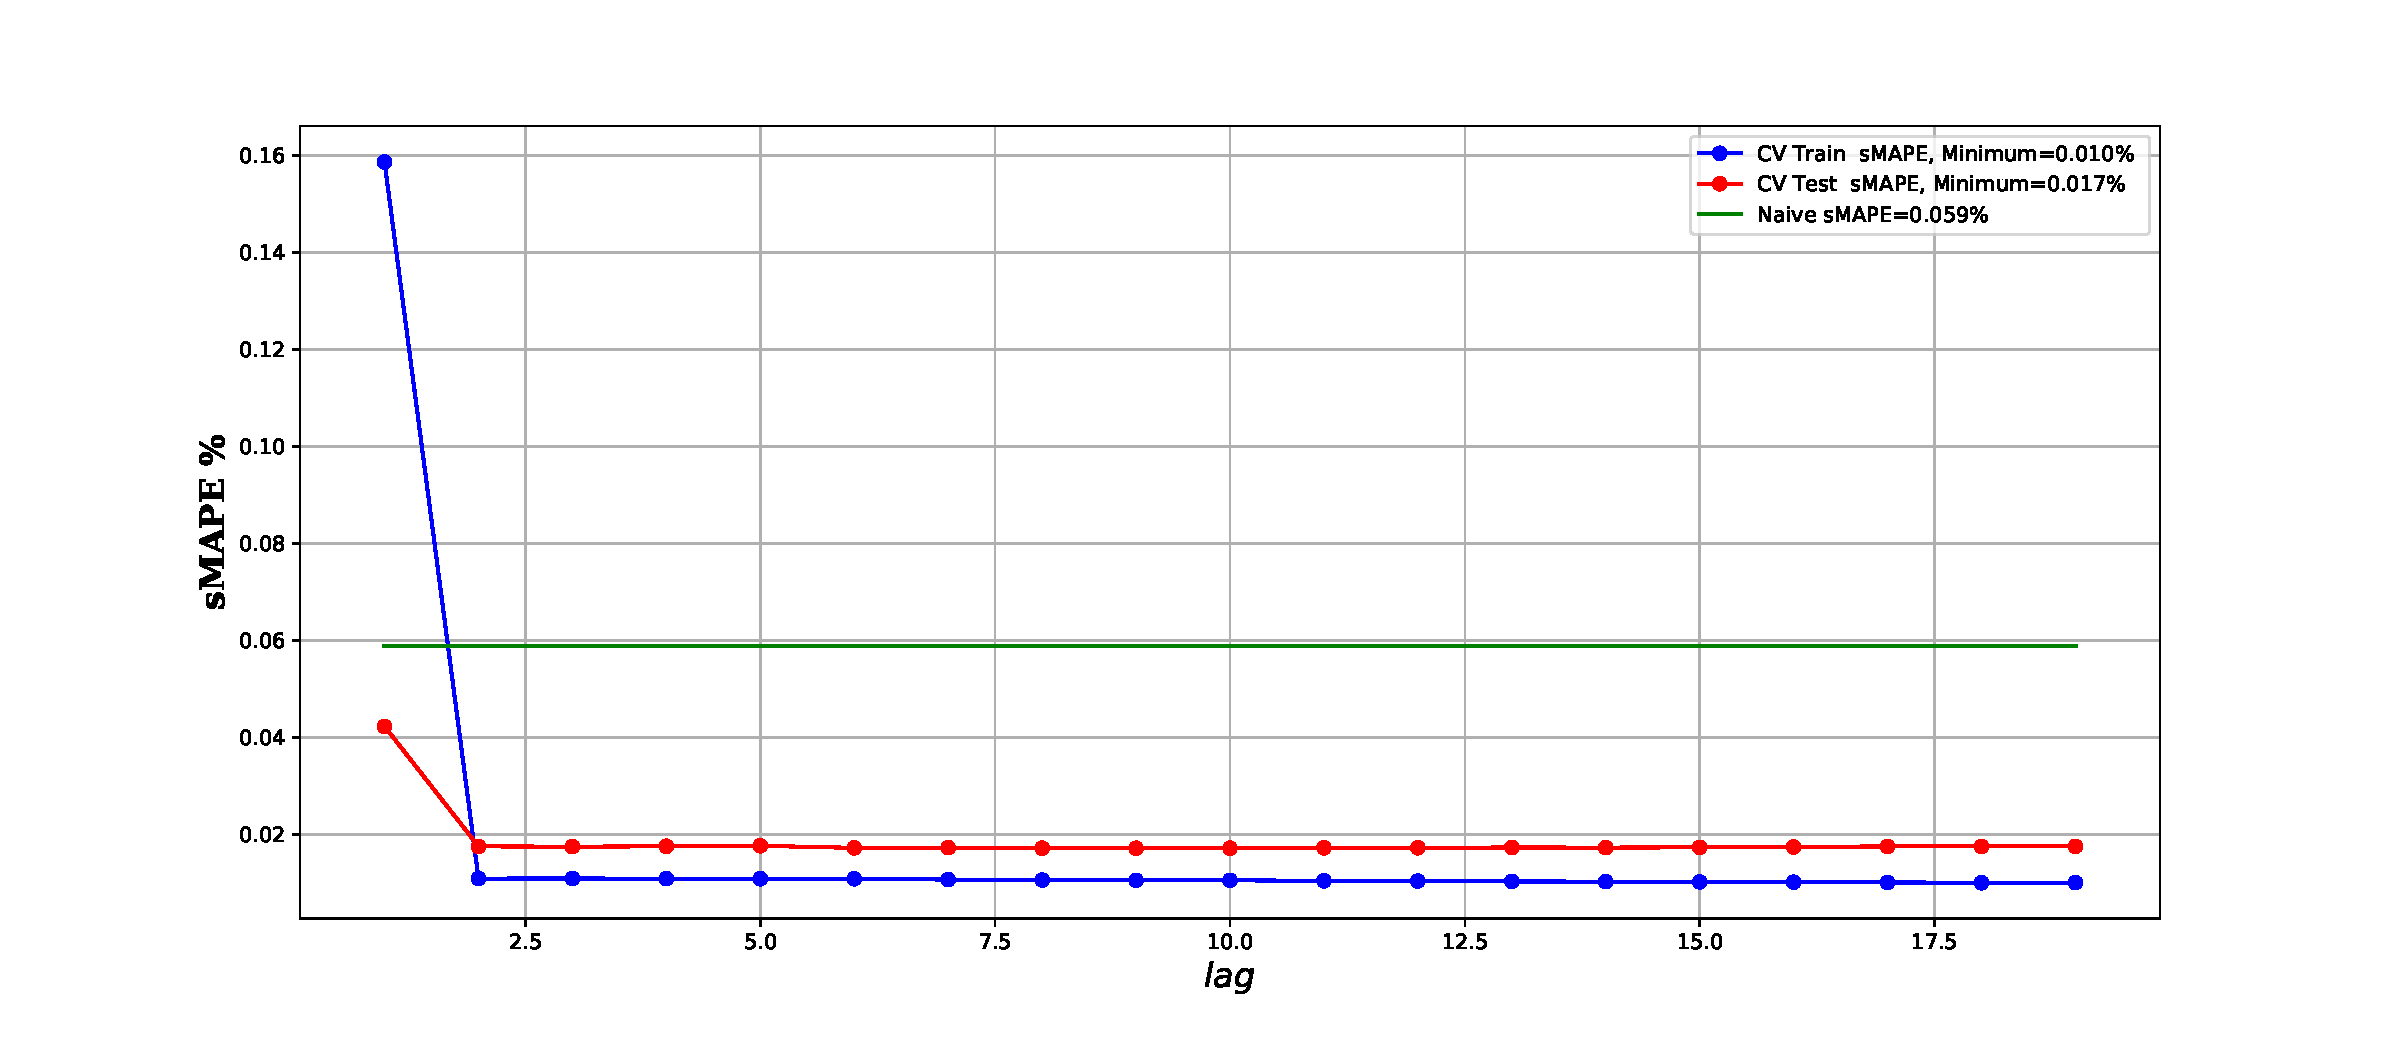
\includegraphics[width=\textwidth]{notebooks/data/trend_sc_1_lag.pdf}
		\caption{\textbf{Random variable} $T_{t}$ \textbf{Model}: Ridge regression. \textbf{$CV_{Rol}$}=100. $\alpha$=0, $\theta$=$lag$, } % For your caption
		\label{fig:trend_sc_1_lag}
	\end{minipage}
	
\end{figure}


In the case of $T^{mv}$ is clear that any model with more than one $lag$ outperforms the naive forecast (green line) however for $E$ only the $lag_{max}=3$ comes close to the naive forecast. In general terms the complexity of this model is giving by the parameter $lag_{max}$ into consideration and as expected the training error is reduced while the complexity of the model increases, the test error, on the other hand, tends to increase. It can also be observed that the variance training $sMAPE$ is very small, $0.054\%$ for $E$ and $0.001\%$ for $T$ which plays in favor of the argument that this problem is very well protected against overfitting \footnote{At least the way it was implemented here.}. In the next optimization, we experiment with $\alpha$ to see if this is the case. \\

\begin{figure}[h!]
	\centering
	\begin{minipage}[b]{\textwidth}
		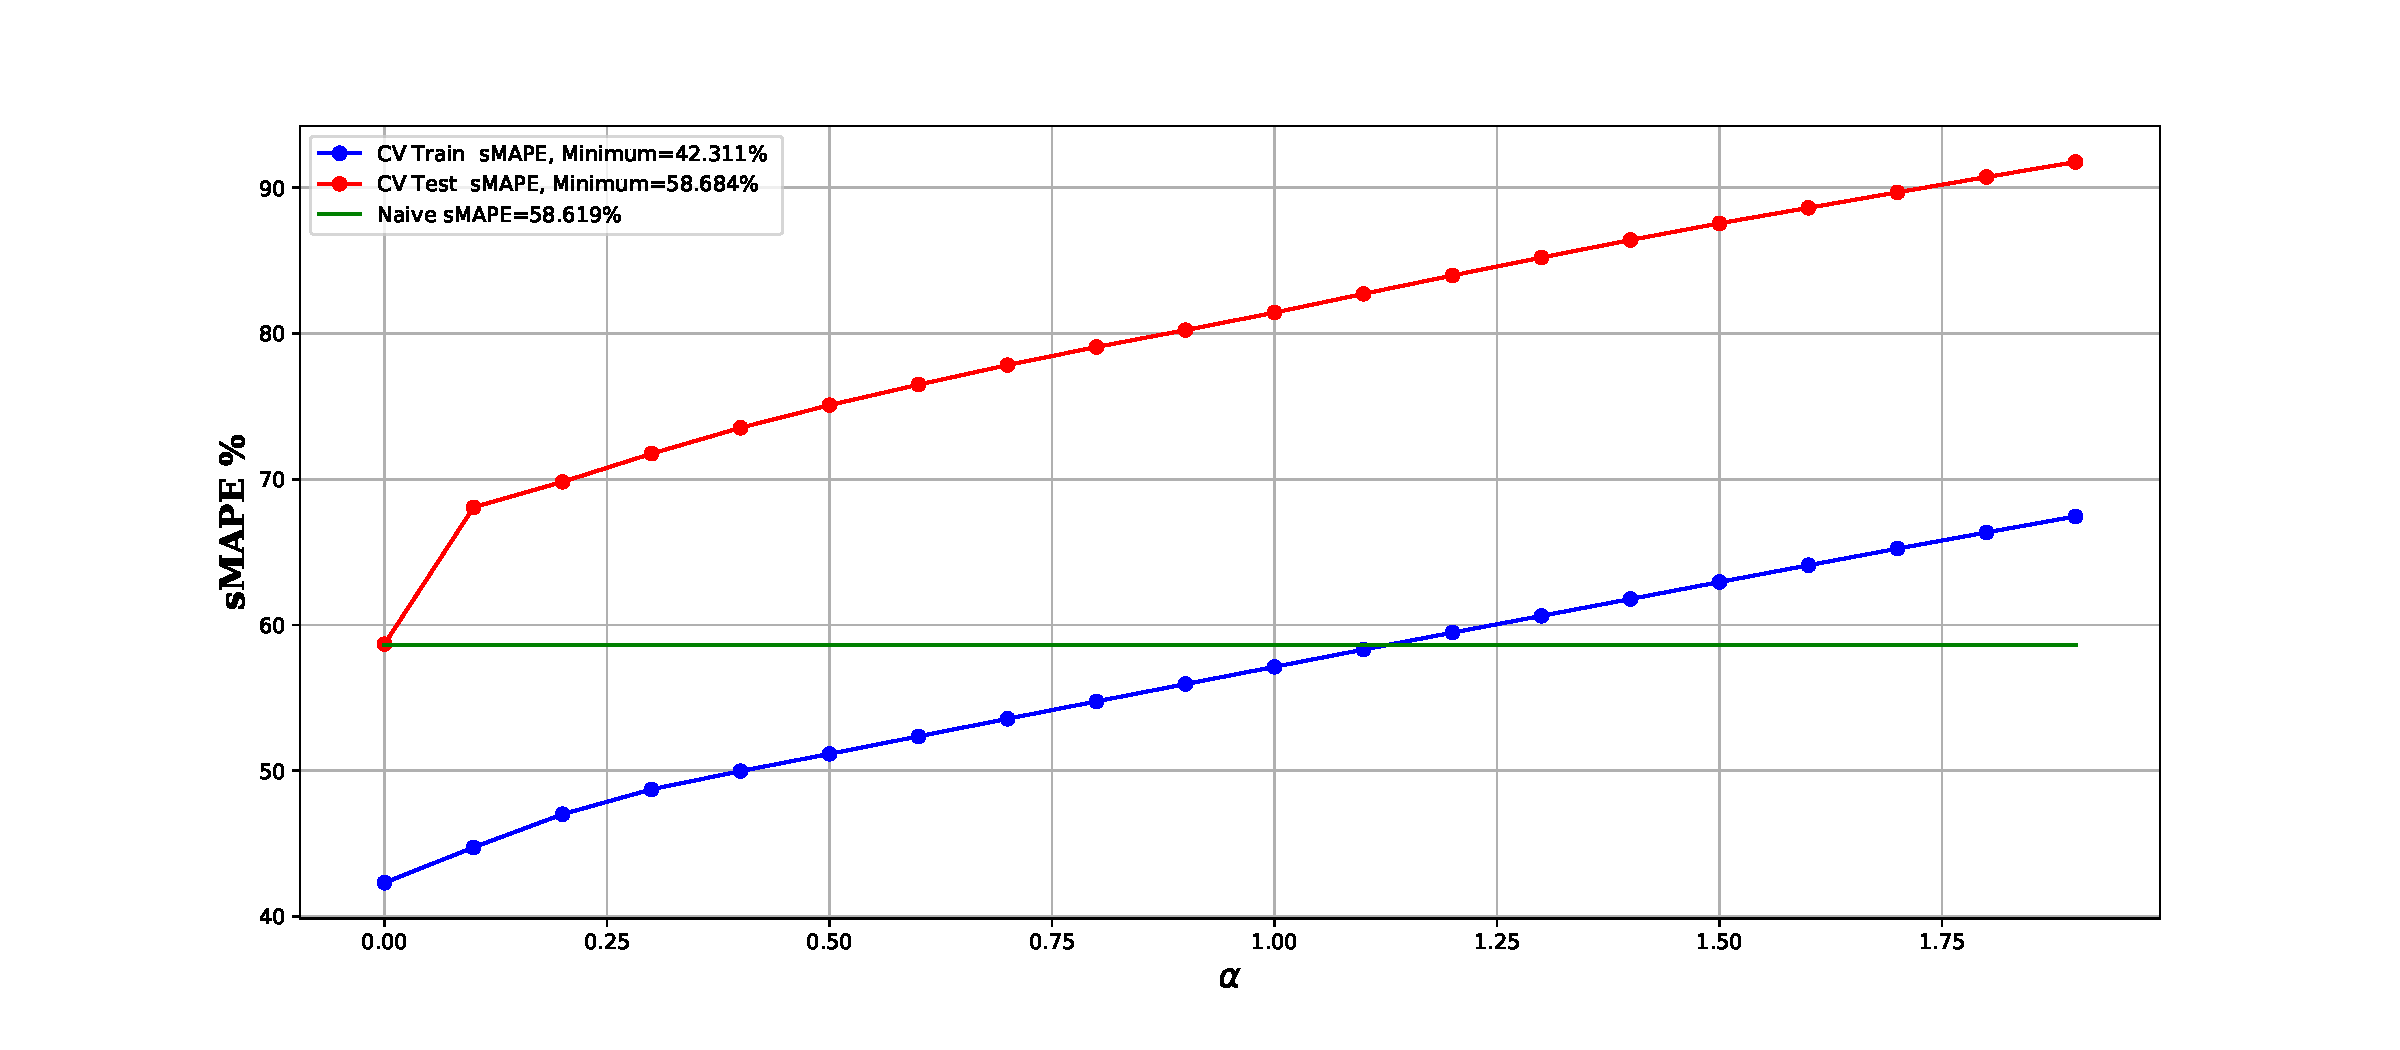
\includegraphics[width=\textwidth]{notebooks/data/error_sc_1_alpha.pdf}
		\caption{\textbf{Random variable} $E_{t}$ \textbf{Model}: Ridge regression. \textbf{$CV_{Rol}$}=100. $lag_{max}=3$, $\theta$=$\alpha$, }
		\label{fig:error_sc_1_alpha}
	\end{minipage}
	\hfill
	\begin{minipage}[b]{\textwidth}
		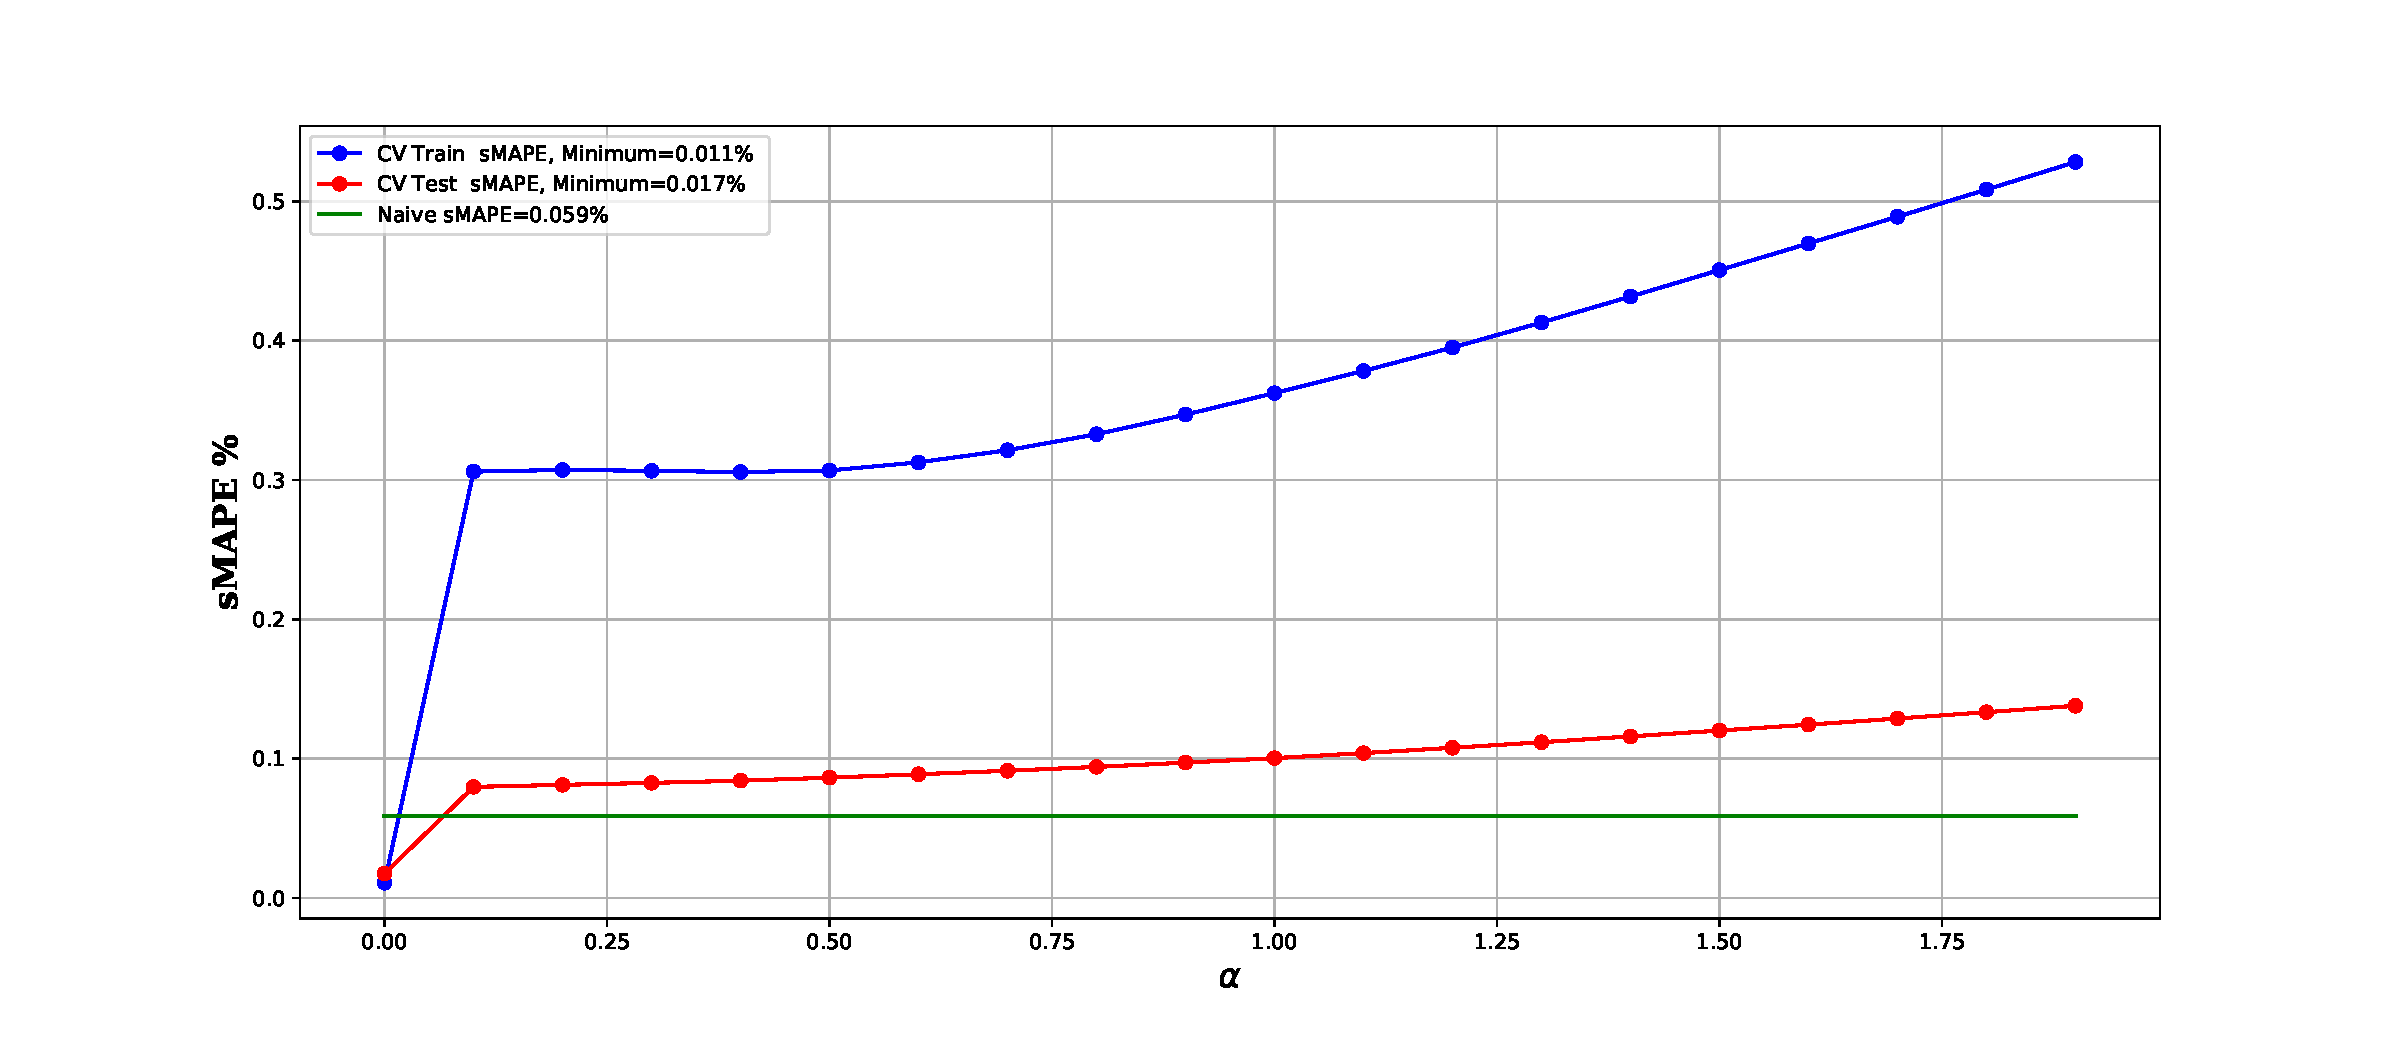
\includegraphics[width=\textwidth]{notebooks/data/trend_sc_1_alpha.pdf}
		\caption{\textbf{Random variable} $T_{t}$ \textbf{Model}: Ridge regression. \textbf{$CV_{Rol}$}=100. $lag_{max}=3$, $\theta$=$\alpha$, }  % For your caption
		\label{fig:trend_sc_1_alpha}
	\end{minipage}
\end{figure}



The minimum testing error is around $58\%$ for  $E$ which is a sign that perhaps the real underlying probability distribution $P$ for our problem is far from linear, it can also be argued that there is not enough information about the phenomena in our data set to estimate the distribution. We explore such questions in the following sections.\\




We now proceed to find the best $\alpha$ giving that $lag_{max}=3$ is the optimal parameter for $E$. For the sake of simplicity, we also set $lag_{max}=3$ to $T^{mv}$. The results can be appreciated in Figure \ref{fig:error_sc_1_alpha} and \ref{fig:trend_sc_1_alpha}.\\ 

The best models for both random variables are the ones with no regularization, as commented in the previous sections $\alpha$ is used to decrease the variance on the training set while theoretically increasing the generalization performance, nonetheless in our particular task the model has already low variance before using $\alpha$, so its implementation is actually detrimental for performance. Another reason for this behavior can be attributed, in the case of $E_{t}$, to a very none linear problem, so that linear regression is not able to properly learn the patterns in the training data. \\



\subsubsection{Single Layer Perceptron for $E$}

A linear decision function was not appropriated for the variable $E$, so a non linear method, namely \emph{Single Layer Perceptron}  $\mathcal{N}:\mathbb{R}^{lag_{max}} \rightarrow \mathbb{R}$ in tested in this section. This machine learning algorithm is characterized by two weighting matrices $W_{0} \in \mathbb{R}^{H_{units}\times lag_{max}} $ and $W_{1} \in \mathbb{R}^{1 \times H_{units}}$ that connect the input feature vector $\mathbb{R}^{lag_{max}}$ to a hidden layer that contains $H_{units} \in N$ hidden units (a hidden layer can be view as column vector of $H_{units}$ components). Each of the hidden units is a linear combination of the connection dictated by the weighting matrix with the previous layer; this linear combination is passed as an argument to the nonlinear activation function, known as sigmoids, such as the hyperbolic tangent $tanh$ used in the present development. 

\begin{figure}[htpb!] % Defines figure environment
	\centering % Centers your figure
	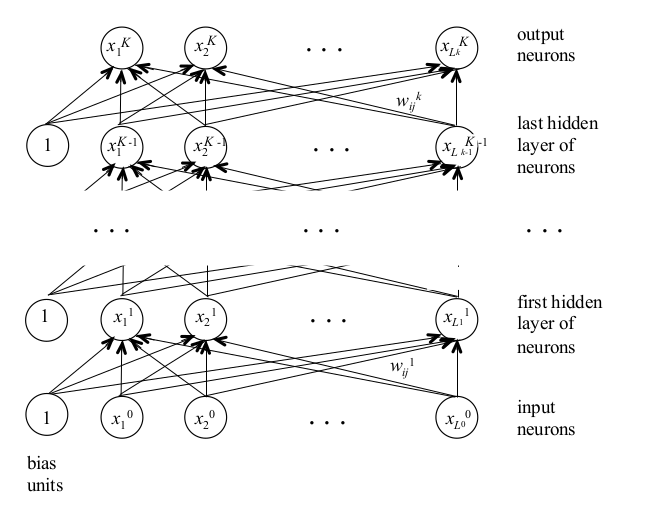
\includegraphics[width=0.4\textwidth]{notebooks/data/nn.png} % Includes your figure and defines %the size
	\caption{Schematic view of a general feed forward neuron network. Taken from  \cite{ml_jacobs_h}.} % For your caption
	\label{fig:nn} % If you want to label your figure for in-text references
\end{figure}

We begin this modeling task by trying to implement the \emph{gradient-decent} algorithm explained in Machine learning lecture notes, where the matrices $W_{1}$  and $W_{0}$ are randomly initialized and the \emph{back propagation} algorithm is used to estimate the gradient of the loss function, which will in term be used to solve the minimization of loss problem. In this approach an update of the weighting matrices occurs once all the data point have been cover and is proportional to a \emph{learning rate} $\lambda \in \mathbb{R}^{>0}$, if this update occurs before all the data points have been covered, we have \emph{batch gradient descent} implementation. Unfortunately, this implementation uses standard $cpu$ hardware to make gradient updates (also know as \emph{epochs}), making it very slow to converge. To bypass this inconvenience we decided to use \emph{Keras} with \emph{Tensor-flow}\cite{chollet2015keras} to speed up the convergence time using \emph{gpu} hardware while maintaining the same theoretical premises explained in the lecture notes, this means that \emph{gradient descent} was forced(by setting the scholastic gradient descent with batch size equal to the number of data points, and preventing the shuffling of data points) with a fixed  $\lambda$.\\

We set somewhat arbitrarily the rule in Equation \ref{eq:4_7}, to have a simple guide for testing some models.


\begin{equation}
H_{units}*lag_{max}+H_{units}<N/10
\label{eq:4_7}
\end{equation}

Following equation \ref{eq:4_7} is possible to reasonable select a maximum number of units in the hidden layer. Beyond this point setting a testing environment as the one shown in Ridge regression is futile (please see \textit{Comments on $\Theta$} section). Table \ref{table:mlp_at} contains some of the parameters implemented  for $\mathcal{N}$ ordered by test $\%(sMAPE)$, we see that best parameters seems to be $H_{units}=6$, $Lag_{max}=15$ which is $3.64\%$  better than the \textit{Naive forecast sMAPE: 58.61 $\%$.}\\


\begin{table}[h!]
	\begin{center}
		\begin{tabular}{||c c c c c c||} 
			\hline
			$H_{units}$ &$Lag_{max}$ &$\lambda$ & $Iter$ & $Train(sMAPE)$ & $Test(sMAPE)$ \\ [0.5ex] 
			\hline\hline
			6& 15 & 0.1 & 100000 & $42.83\%$ & $54.97\%$ \\ 
			\hline
			6& 15 & 0.1 & 12000 & $43.05\%$ & $56.47\%$ \\ 
			\hline
			50& 1 & 0.1 & 2000 & $43.88\%$ & $56.68\%$ \\ 
			\hline
			16& 5 & 0.1 & 8000 & $42.30\%$ & $57.17\%$ \\ 
			\hline
			27& 3 & 0.1 & 8000 & $42.07\%$ & $57.85\%$ \\ 
			\hline
			12& 7 & 0.1 & 5000 & $42.63\%$ & $59.39\%$ \\ 
			\hline
			33& 2 & 0.5 & 3000 & $42.59\%$ & $59.49\%$ \\
			\hline
			12& 7 & 0.1 & 10000 & $43.37\%$ &$59.92\%$ \\ 
			\hline
			12& 7 & 0.1 & 9000 & $42.41\%$ & $60.27\%$ \\ 
			\hline
			25& 3 & 0.01 & 10000 & $64.68\%$ & $64.68\%$ \\ 
			\hline
			9& 10 & 0.01 & 10000 & $49.84\%$ & $68.54\%$ \\ 
			\hline
		\end{tabular}
		\caption{ $\Theta$ Variation. \textit{solver}: Gradient decent. $W_{o}$: normal distributed (Random seed:7). $f_{act}$: $tanh$. \textit{Naive forecast sMAPE: 58.61$\%$}}
		\label{table:mlp_at}
	\end{center}
\end{table}

\textbf{some comments on $\Theta$}
\begin{itemize}
	\item A rational approach would be to increment one by one the number of units in the hidden layer and then evaluate the cross-validation error. Each of this steps would have the same $\lambda$ as well as the same number of iterations to be interpretable by us, however as we increase the number hidden units, keeping the same $\lambda$ might not be appropriate giving that the vector of parameters $\phi$ has increased in dimension, this increase might cause the gradient descent update of state not as effective, which in term would might cause the number of iterations to be insufficient for convergence.
	\item Setting extreme small values $\lambda$ to cover most scenarios requires massive amount computational time, setting $\lambda$ relative big, will cause not convergence.
	\item Giving the random nature of the initialization of weighting matrices and the fact that gradient descent is very likely to wander around local minimal, compering in such straight forwards different manner architecture seems like undefined endeavor.
\end{itemize}




\subsection{Decomposition, Simple Exponential Smoothing based}


For simple exponential smoothing\footnote{Implemented using \cite{Statsmodels}} trend calculation, the parameter $\beta$ in Equation \ref{eq:SES} determines the amount of exponential decrease of the influence of past observations over the current time step. For small values of $\beta$ more history of past observations weight in the current time step value, whereas a large $\beta$ would give more influence of observations near the present. In Figure \ref{fig:tren_simple_exp} we can see different values of the smoothing factor $\beta$. A smoothing parameter of 0.5 was selected, and the process of decomposition describe in the previous section was repeated. Note that no attempt for calculating the seasonality was carried since this is a property of the time series itself, independent of the tool used for modeling the trend.

\begin{figure}[h!] % Defines figure environment
	\centering % Centers your figure
	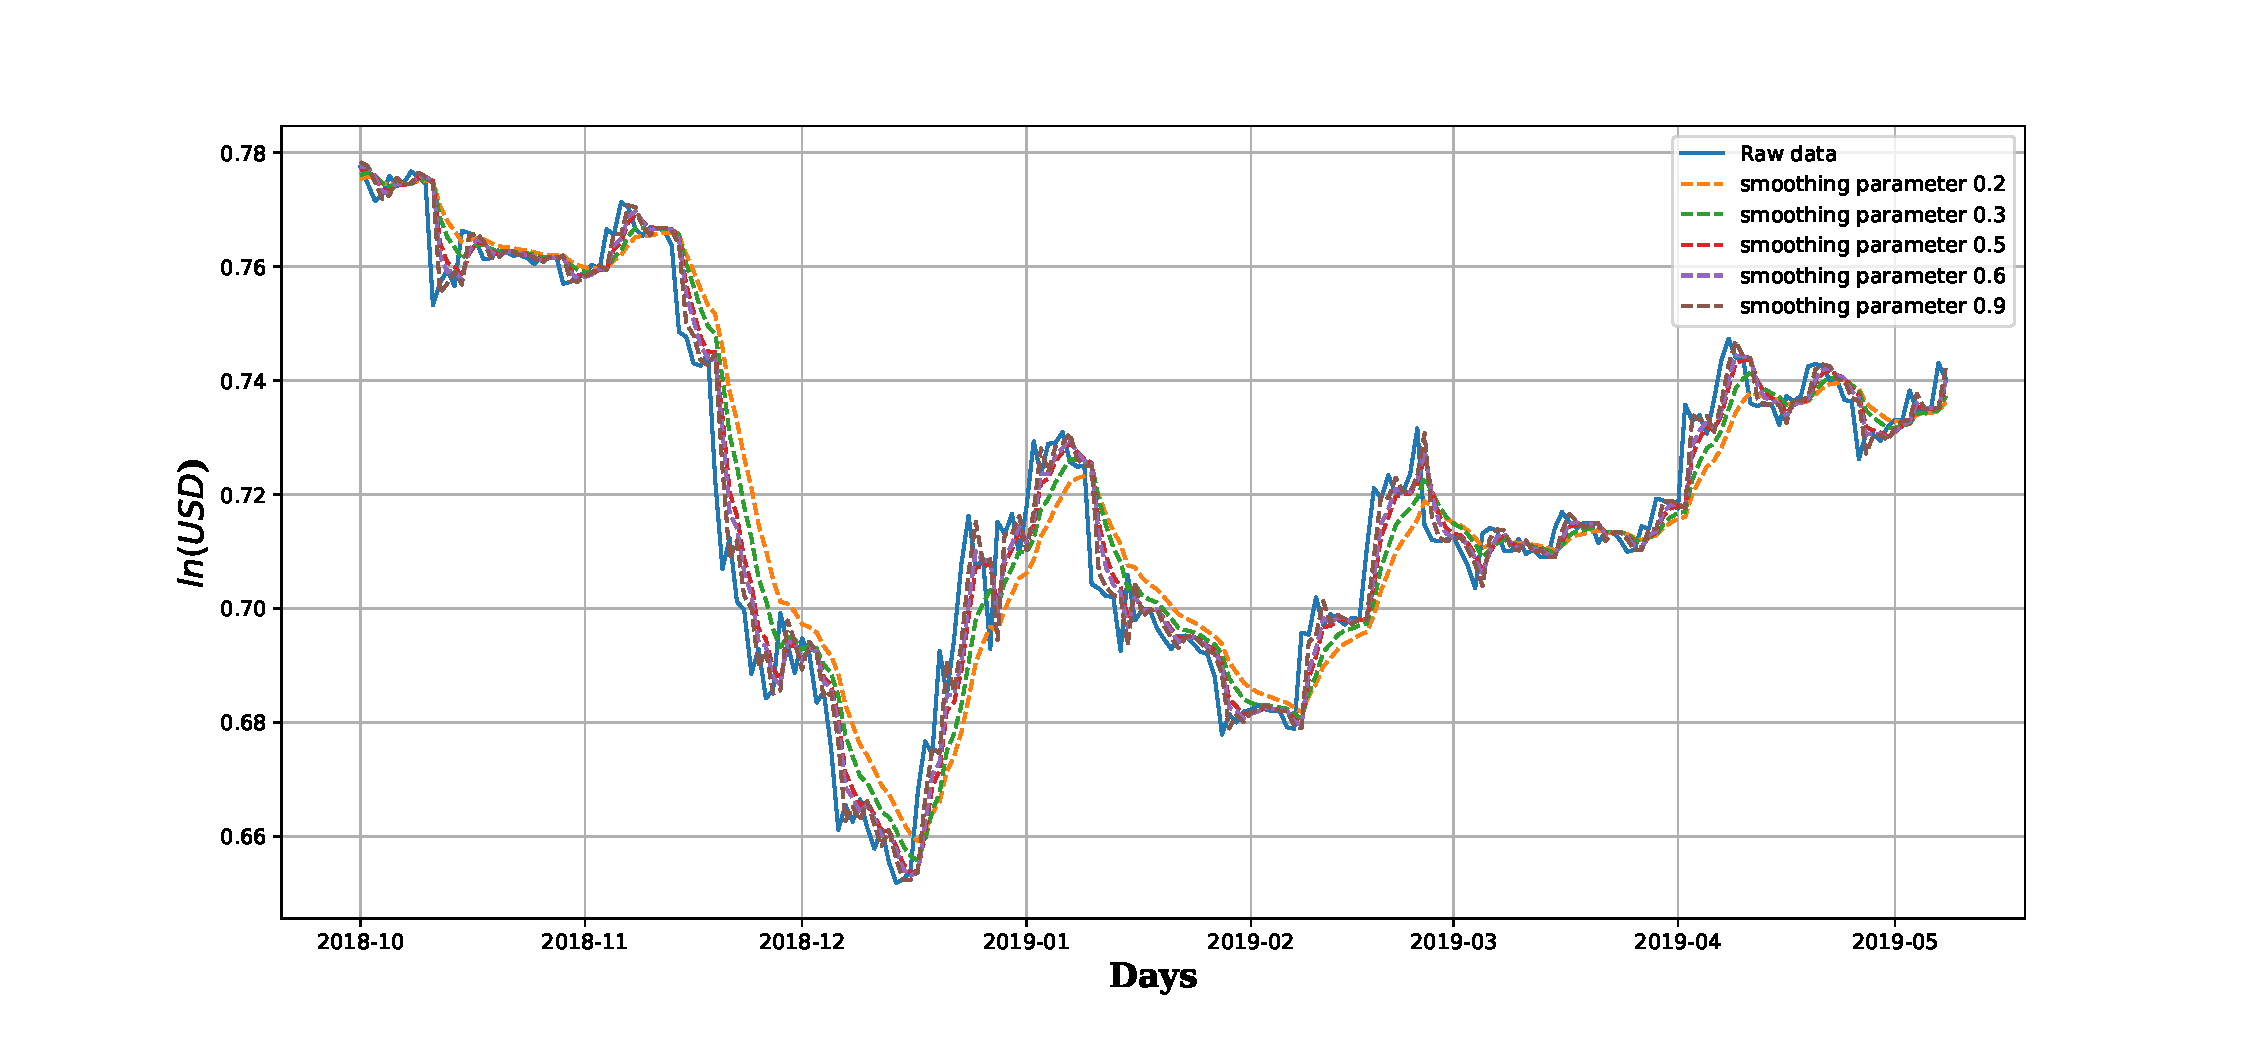
\includegraphics[width=0.75\textwidth]{notebooks/data/trend_SES.pdf} % Includes your figure and defines %the size
	\caption{Simple Exponential Smoothing for year 2019} % For your caption
	\label{fig:tren_simple_exp} % If you want to label your figure for in-text references
\end{figure}

By inspecting Figure \ref{fig:tren_simple_exp_error} where the derived error $E^{ses}$ is plotted a noise behavior is clearly discernible as consequence we  decided to apply  a two tail statistical test over the null $H_{o}$ that $y=T^{ses}+E^{ses}$ and $y'=T^{ses}$ are in fact the same random variable.

\begin{figure}[h!] % Defines figure environment
	\centering % Centers your figure
	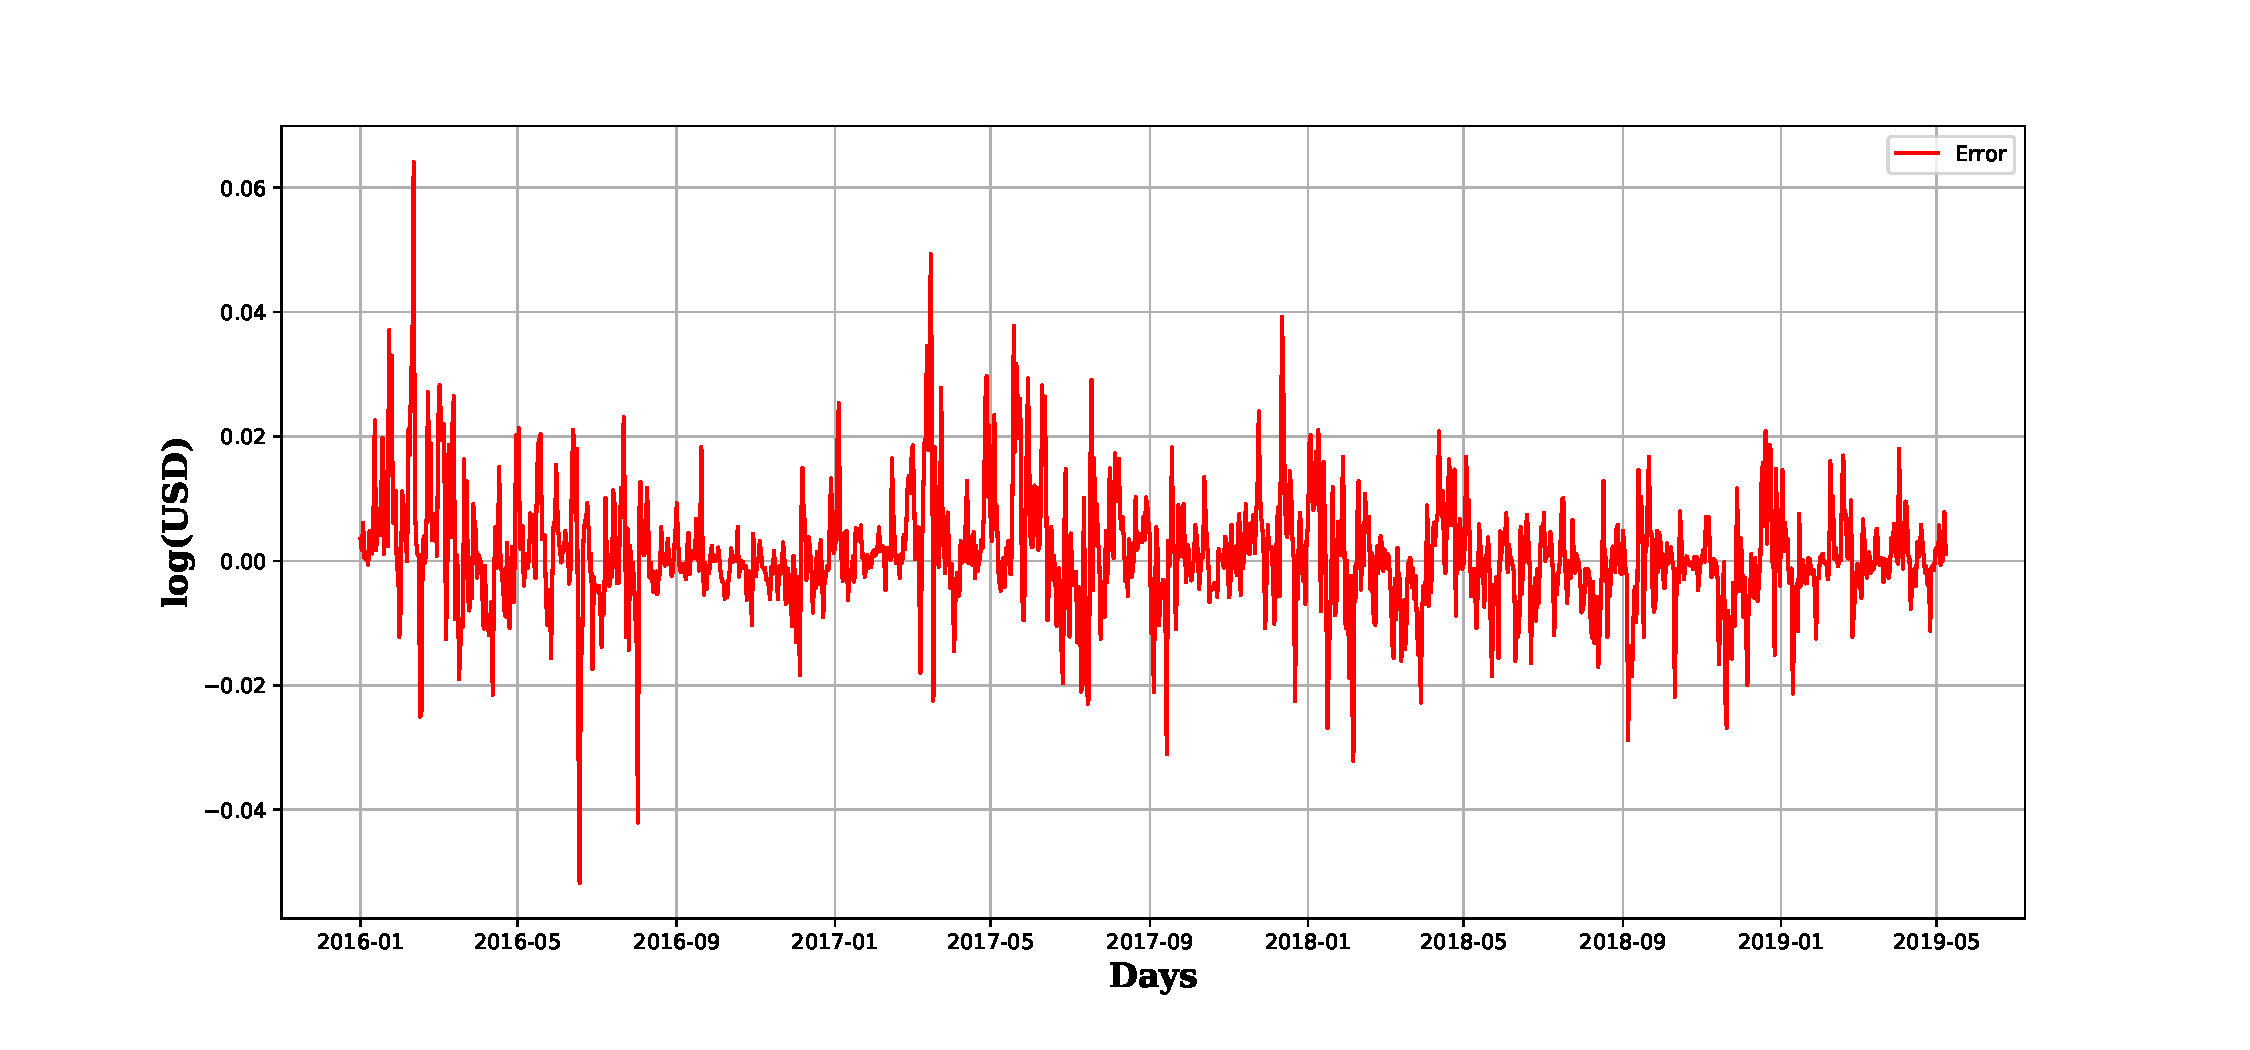
\includegraphics[width=0.85\textwidth]{notebooks/data/Residual_error_u_SES.pdf} % Includes your figure and defines %the size
	\caption{$E_{t}$ Using exponential smoothing for the $T_{t}$} % For your caption
	\label{fig:tren_simple_exp_error} % If you want to label your figure for in-text references
\end{figure}

Table \ref{table:t_test_sms_error} summarizes the t-test. With a p-value so close to 1, it is not possible to reject $H_{o}$.The new relationship becomes $y=T^{ses}$.

\begin{table}[h!]
	\begin{center}
		\begin{tabular}{||c c c||} 
			\hline
			RV & t-value & p-value \\ [0.5ex] 
			\hline\hline
			$y$,$y'$ & 0.11 & 0.90  \\ 
			\hline
		\end{tabular}
		\caption{T-test for Error.}
		\label{table:t_test_sms_error}
	\end{center}
\end{table}


In Figure \ref{fig:trendses} we see cross-validation plot for $lag_{max}$ optimization using Ridge regression, the minimum test $\%sMAPE$ is $0.245\%$. 

\begin{figure}[htpb!] % Defines figure environment
	\centering % Centers your figure
	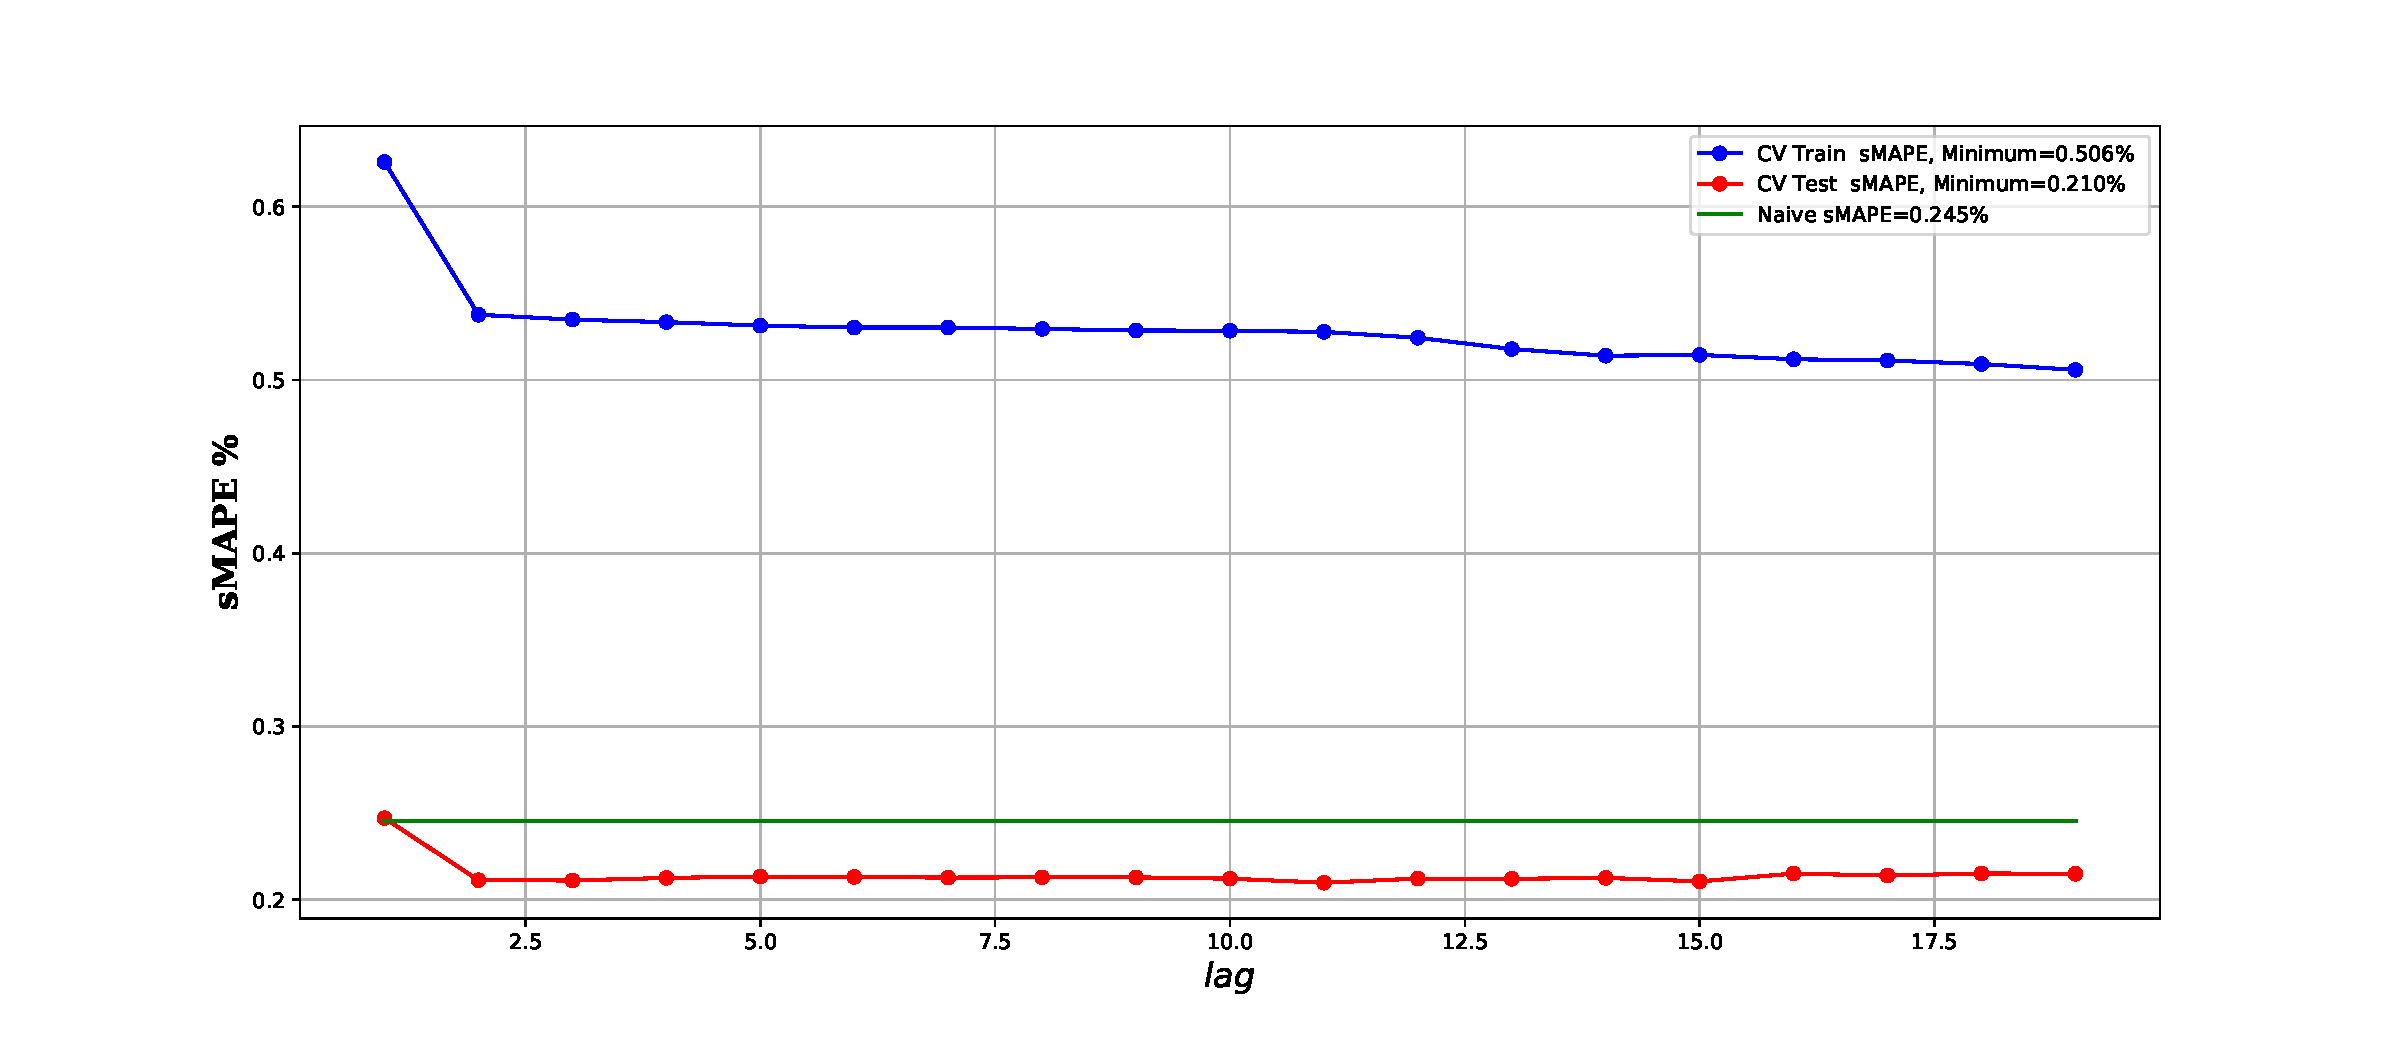
\includegraphics[width=0.8\textwidth]{notebooks/data/trend_ses.pdf} 
	\caption{\textbf{Random variable} $T^{ses}$ from Simple exponential smoothing \textbf{Model}: Ridge regression. \textbf{$CV_{Rol}$}=100. $\alpha$=0, $\theta$=$lag$.  } 
	\label{fig:trendses} % If you want to label your figure for in-text references
\end{figure}

\subsection{Conclusion on Time Series Analysis}

In other to compare both approaches, namely, classical decomposition moving averages(Equation \ref{eq1}) based and exponential smoothings(Equation \ref{eq2}) based, we make consecutive one time step predictions on the year 2019 following Table \ref{table:r1}.

\begin{equation}
y^{mv}_{t}=T^{mv}_{t}+E_{t}
\label{eq1}
\end{equation}

\begin{equation}
y^{ses}_{t}=T^{ses}_{t}
\label{eq2}
\end{equation}

\begin{table}[h!]
	\begin{center}
		\begin{tabular}{||c c c||} 
			\hline
			RV & $\mathcal{D}$ & $lag_{max}$ \\ [0.5ex] 
			\hline\hline
			$T^{mv}$ & Ridge regression ($\alpha =0$) & 2  \\ 
			\hline
			$E$ & Single layer perceptron ($H_{units}=6,\lambda=0.1,Iter=12000$) & 15  \\ 
			\hline
			$T^{ses}$ &  Ridge regression ($\alpha =0$) & 2  \\ 
			\hline
		\end{tabular}
		\caption{Best decision functions per Random variable}
		\label{table:r1}
	\end{center}
\end{table}





\begin{figure}[h!]
	\centering
	\begin{minipage}[b]{\textwidth}
		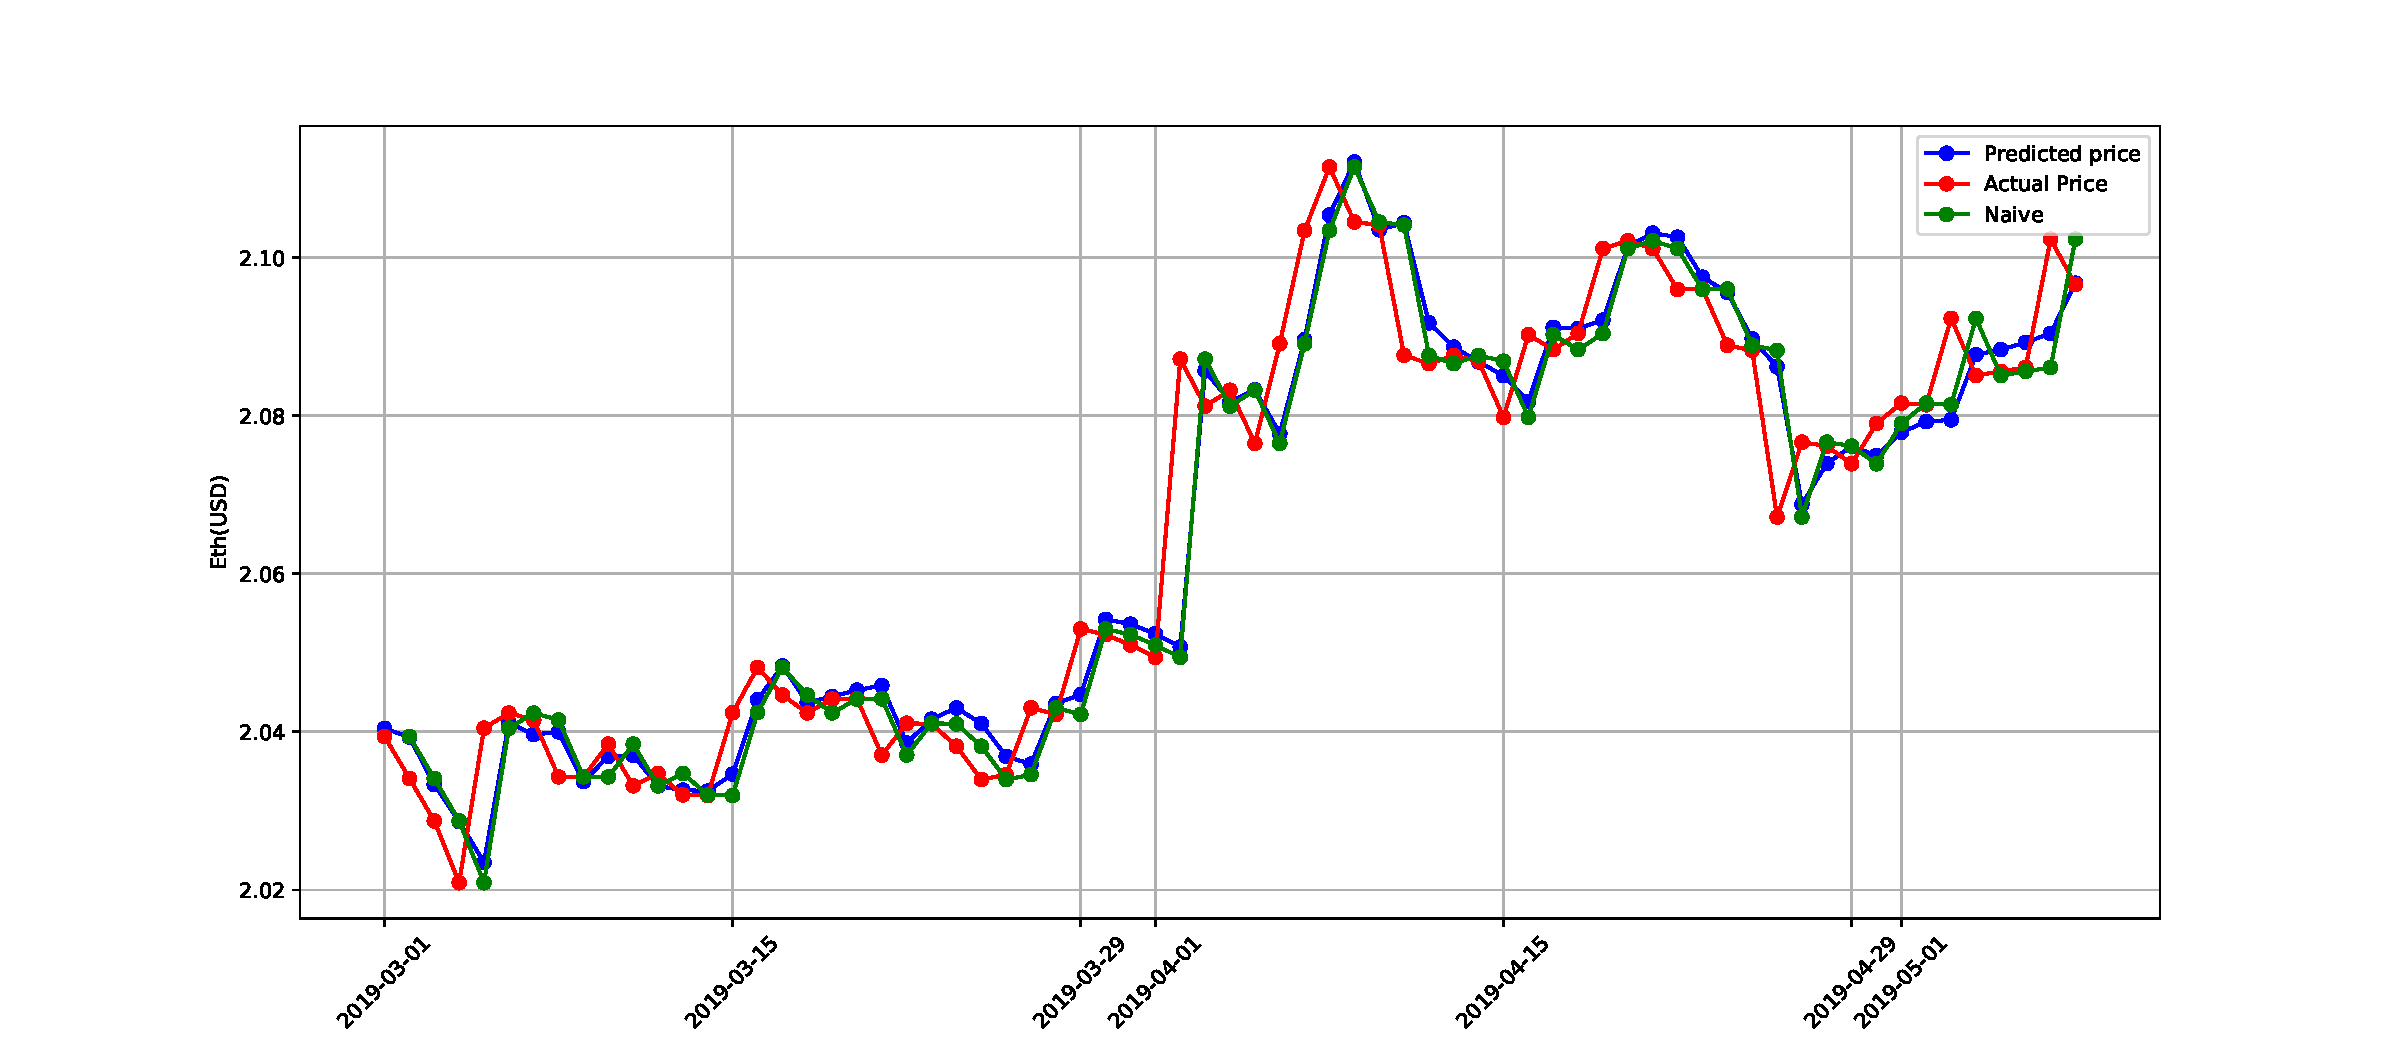
\includegraphics[width=\textwidth]{notebooks/data/pre_2019_mv.pdf}
		\caption{$y^{mv}$ for 2019-03 to 2019-05}
		\label{fig:compa1}
	\end{minipage}
	\hfill
	\begin{minipage}[b]{\textwidth}
		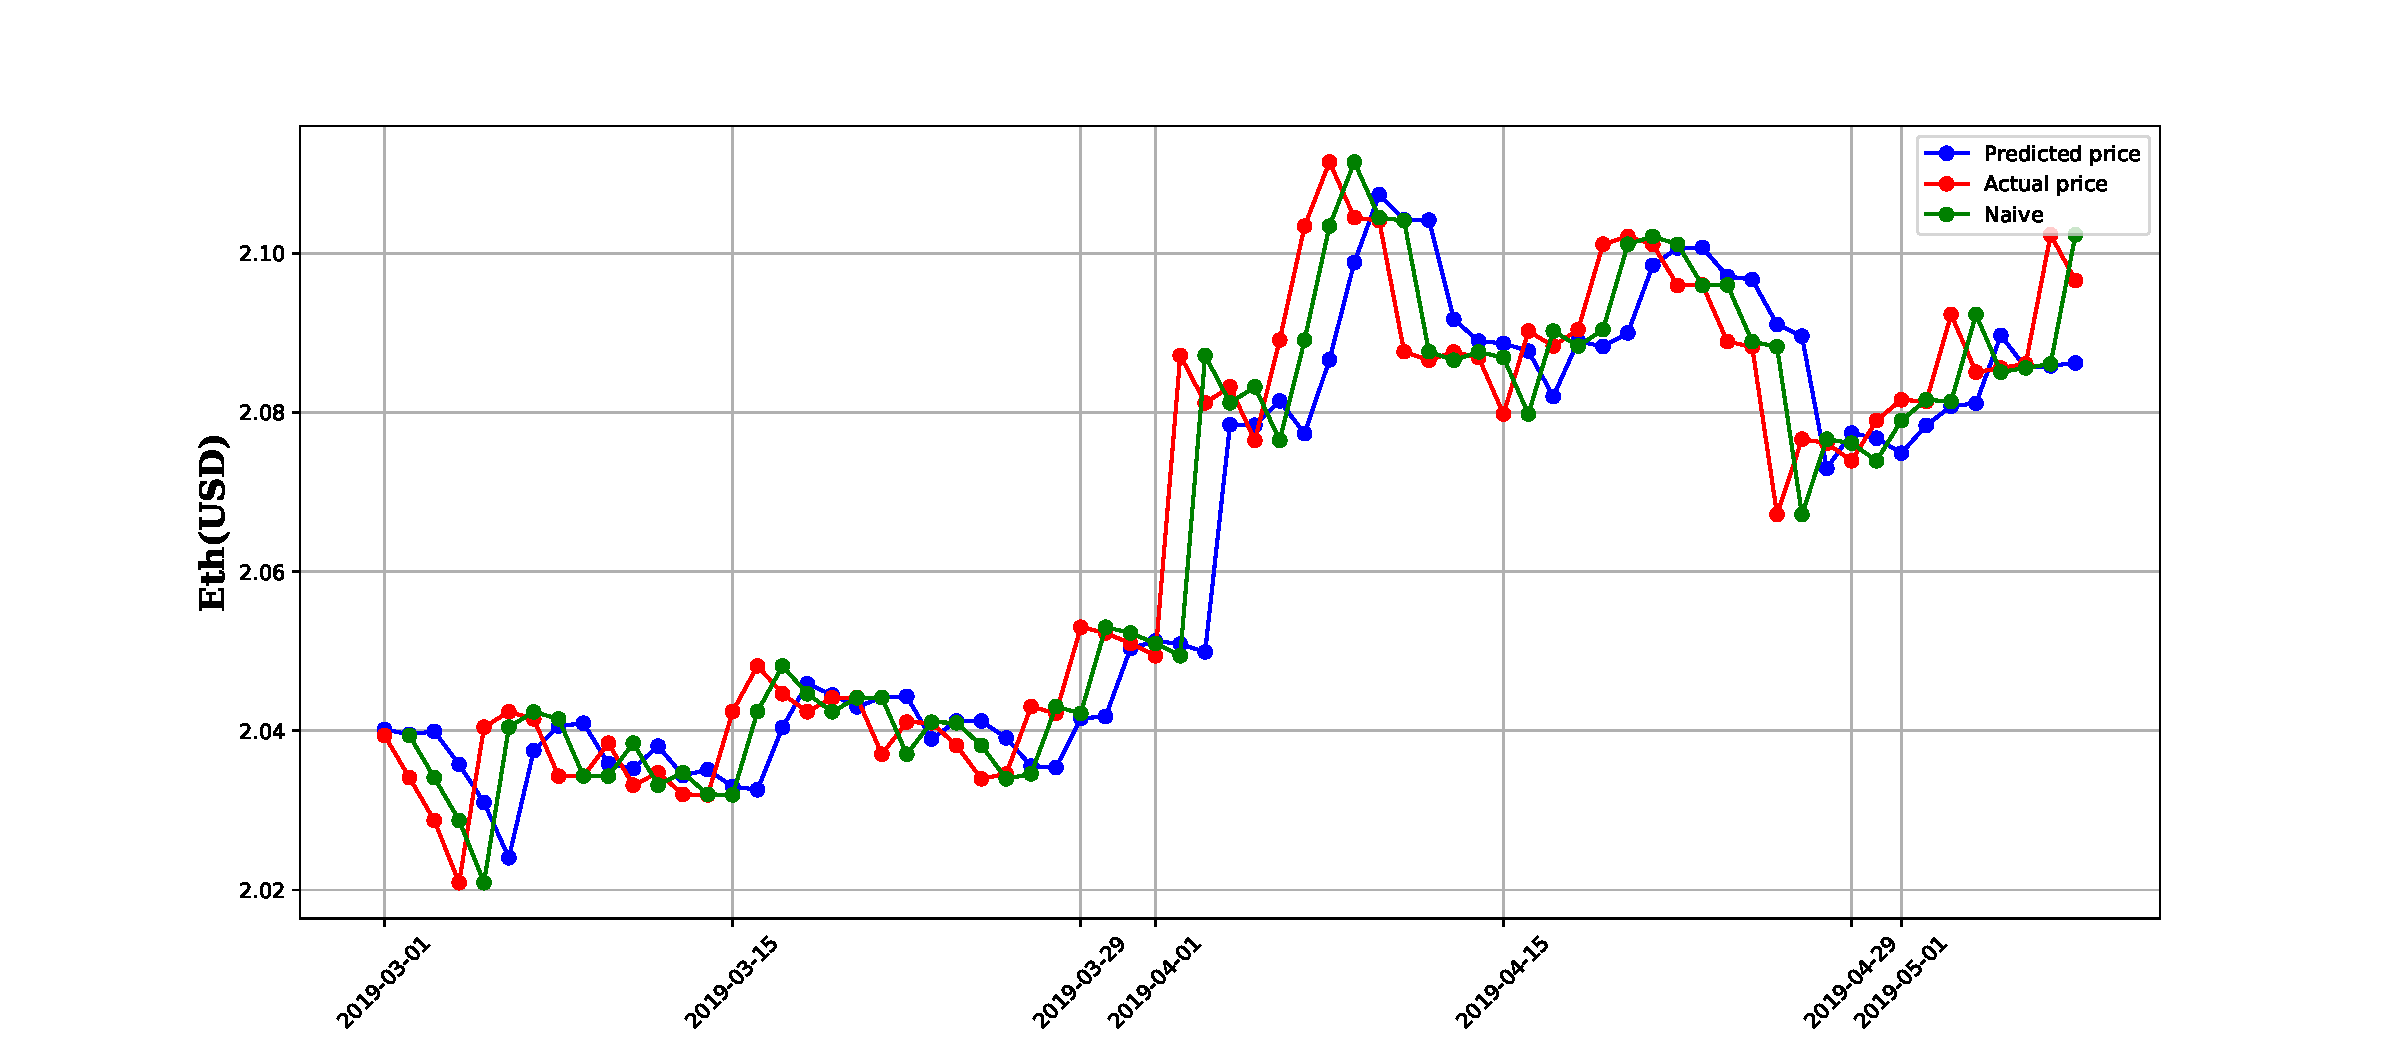
\includegraphics[width=\textwidth]{notebooks/data/pre_2019_ses.pdf}
		\caption{$y^{ses}$ for 2019-03 to 2019-05}
		\label{fig:compa2}
	\end{minipage}
\end{figure}

In Figure \ref{fig:compa1} and \ref{fig:compa2} we plotted the full prediction for the latest three months of 2019. The $\%sMAPE$ for 
$y^{mv}$ is $0.42\%$ for $y^{ses}$ is $0.62\%$ and the naive forecast is $0.44\%$. The final results are somehow disappointing; however, not unexpected since it is a well-accepted fact that markets are irrational in the sense that people behave erratically, and this information is not on the time series itself. This could be further amplified, giving that the cryptocurrency market place is accessible to every individual on the planet, which is not true for other assets, making ever more difficult to predict.


\section{Modeling the Ether price with social media}

We dedicate this section to the inclusion of sentiment in our analysis. As shown in the \emph{Time series} section, the \emph{naive forecast} was never outperformed by a sufficient  $\% sMAPE$  to make the effort of implementing more complex decision functions a reasonable endeavor. In this section, we take the naive forecast as the next day predictor plus a level of hysteria  $hl$ of the previous day.

\begin{equation}
y_{t+1}=y_{t}+ hl_{t}
\label{eq:h}
\end{equation}

Equation \ref{eq:h} tell us that the level of hysteria is defined as $hl_{t}=y_{t+1}-y_{t}$. We also theorized that this random variable is not time dependent and that it is the direct consequence of what people express in social media. A final extra factor is the transitions per day $T_{r}$, which we believe is an indicator of the next volatility, the idea is that when a cryptocurrency owner start moving their digitals access over the blockchain from private wallets to exchange wallets, for example, it seems reasonable to think they are getting ready to sell it in exchange for \emph{fiat} as USD, which may put extra pressure over the price according to supply and demand schema. Combining all this hypothesis we arrive at Equation \ref{eq:h2} where $Tr$ is the number of transactions per day, $I$ is popularity on Google search, and $Tw$ is the popularity score on Twitter, for more details over these variables please see section 1.3.

\begin{equation}
hl_{t}=y_{t+1}-y_{t}=f(Tr_{t},I_{t},Tw_{t})
\label{eq:h2}
\end{equation}



A \emph{Decision tree regressor} is a supervised machine learning algorithm that splits the target value space into sectors called \emph{leafs} by continuously splitting the feature value space into binary \emph{branches}. By increasing the maximum level of binary splitting of the features, we get more leaves or terminal nodes, meaning that the hypercube containing target variable get smaller producing easily overfitted models, for this reason, Decision Trees are considered weak estimators. \emph{Assembly methods} as \emph{Boosting} combine many of those weak estimators in a sequence based on the residual of the previous one. A complete technical explanation can be found in \cite{james2013introduction}. As explain section 1.2, we only had data for social media analysis from 2018-01-19 to 2018-12-03 from 2019-03-16 to 2019-05-01. Since the data was split in this manner, we decided to train \emph{Boosting Decision tree regressor}\footnote{ We used the sklearn implementation in \cite{scikitlearn_bo} } on the data 2018 data interval, and then run a single test of the 2019 range. For parameter optimization, we used grid search sklearn implementation \cite{scikitlearn_grid}.\\

\textbf{Parameters of grid search:}

\begin{itemize}
	\item \emph{learning rate}: 0.01,0.02,0.03
	\item \emph{max depth}:  20,25,30,35 
	\item \emph{n estimators}: 5,10,25,50
\end{itemize}


where the  \emph{learning rate} is the gradient proportional constant for minimizing the loss function in the case de mean square error on each subsequent tree. \emph{max depth} is the maximum level of splitting of the feature vectors per weak estimator, and \emph{n estimators} is the number of weak estimators to use. Using cross 2-fold cross validation we the best parameters are: \emph{learning rate}: 0.01, \emph{max depth}: 25, \emph{n estimators}: 5.



\begin{figure}[h!]
	\centering
	\begin{minipage}[b]{0.8\textwidth}
		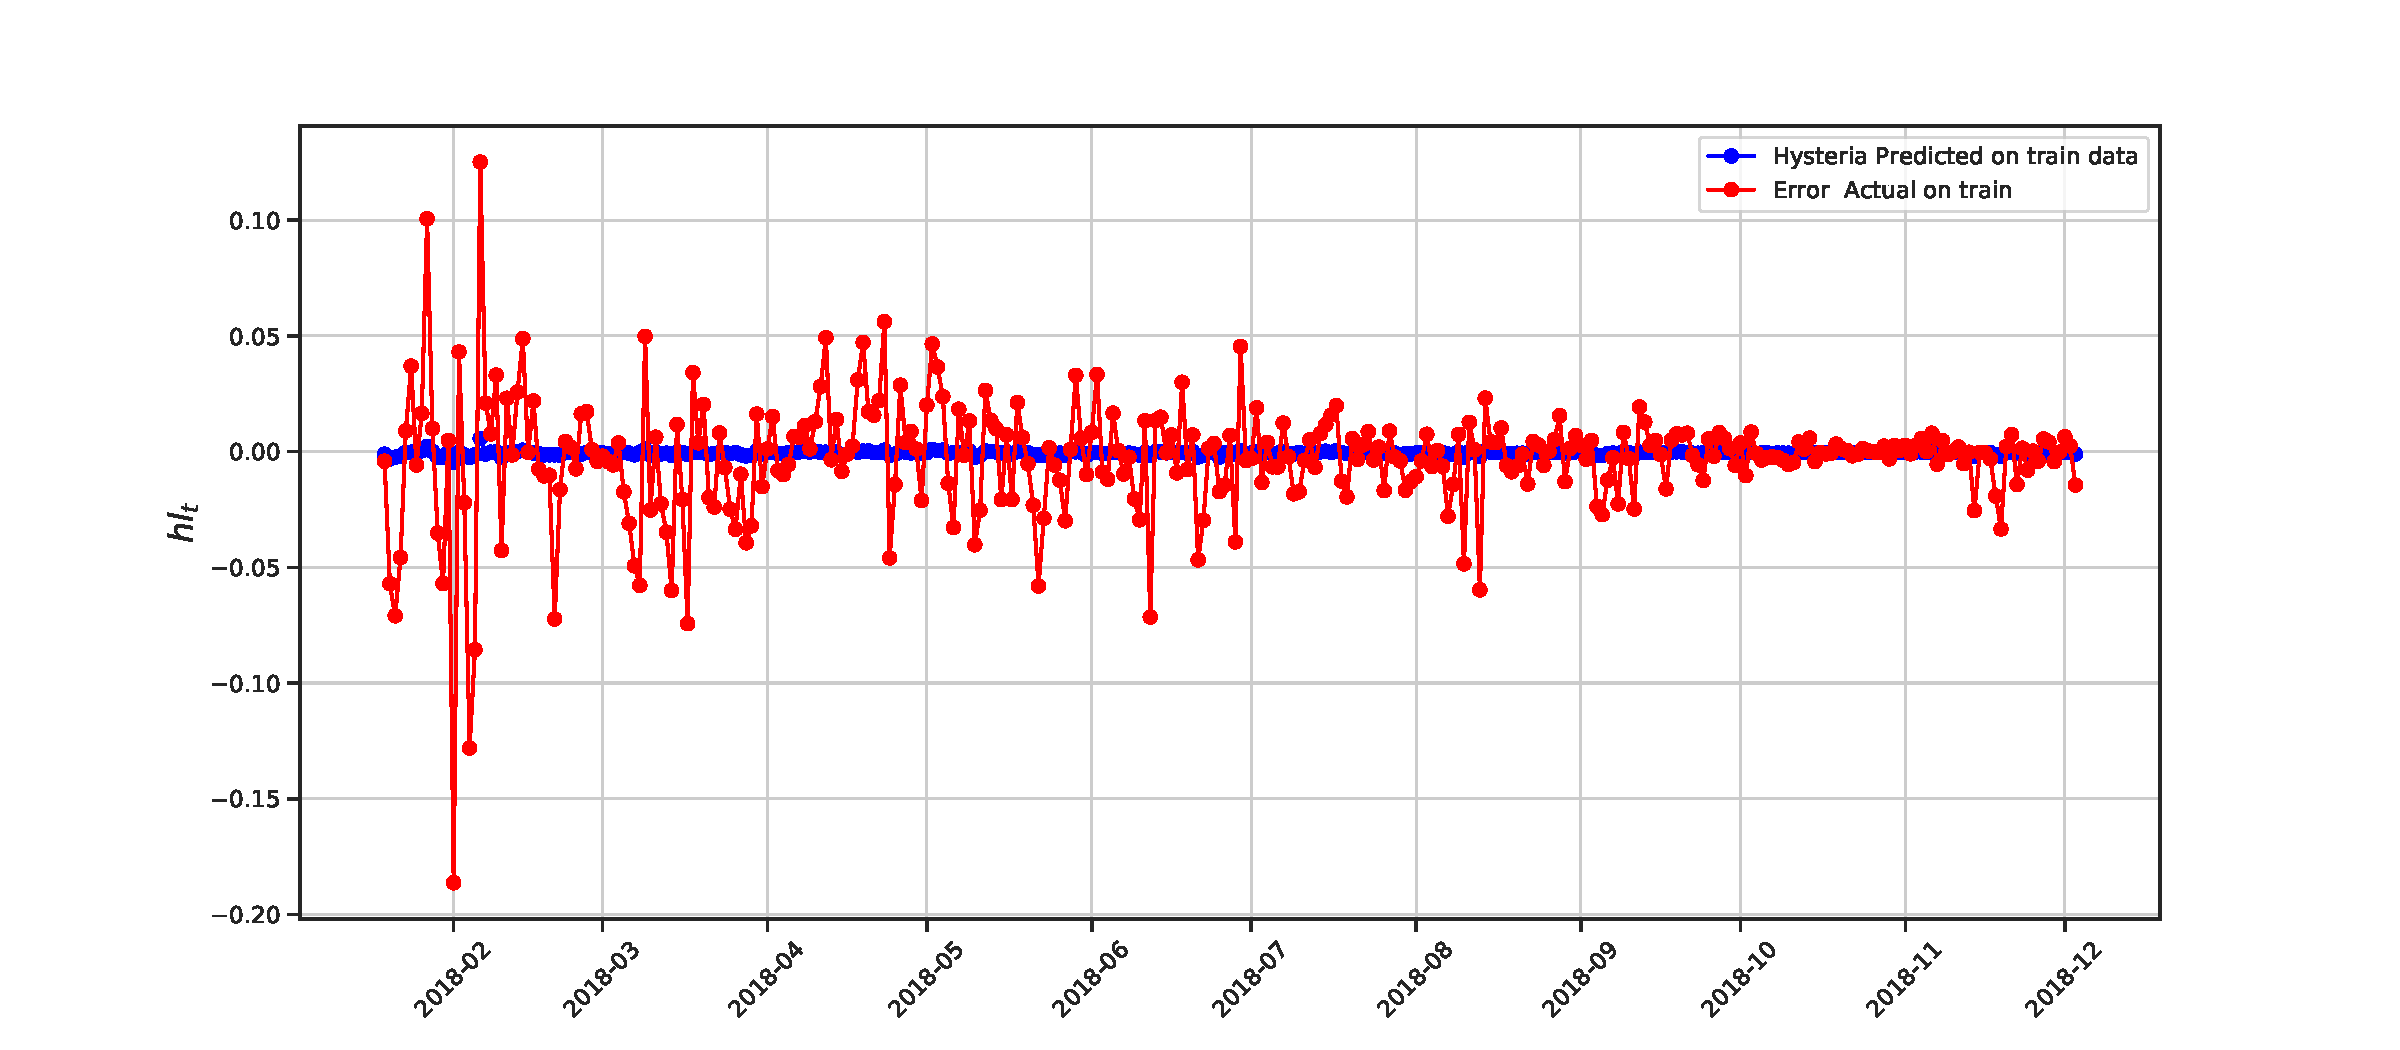
\includegraphics[width=0.9\textwidth]{notebooks/data/2018_hys_senti.pdf}
		\caption{ $hl_{t}$ for 2018-01-19  to  2018-12-03 training set.}
		\label{fig:sent2018}
	\end{minipage}
	\hfill
	\begin{minipage}[b]{0.8\textwidth}
		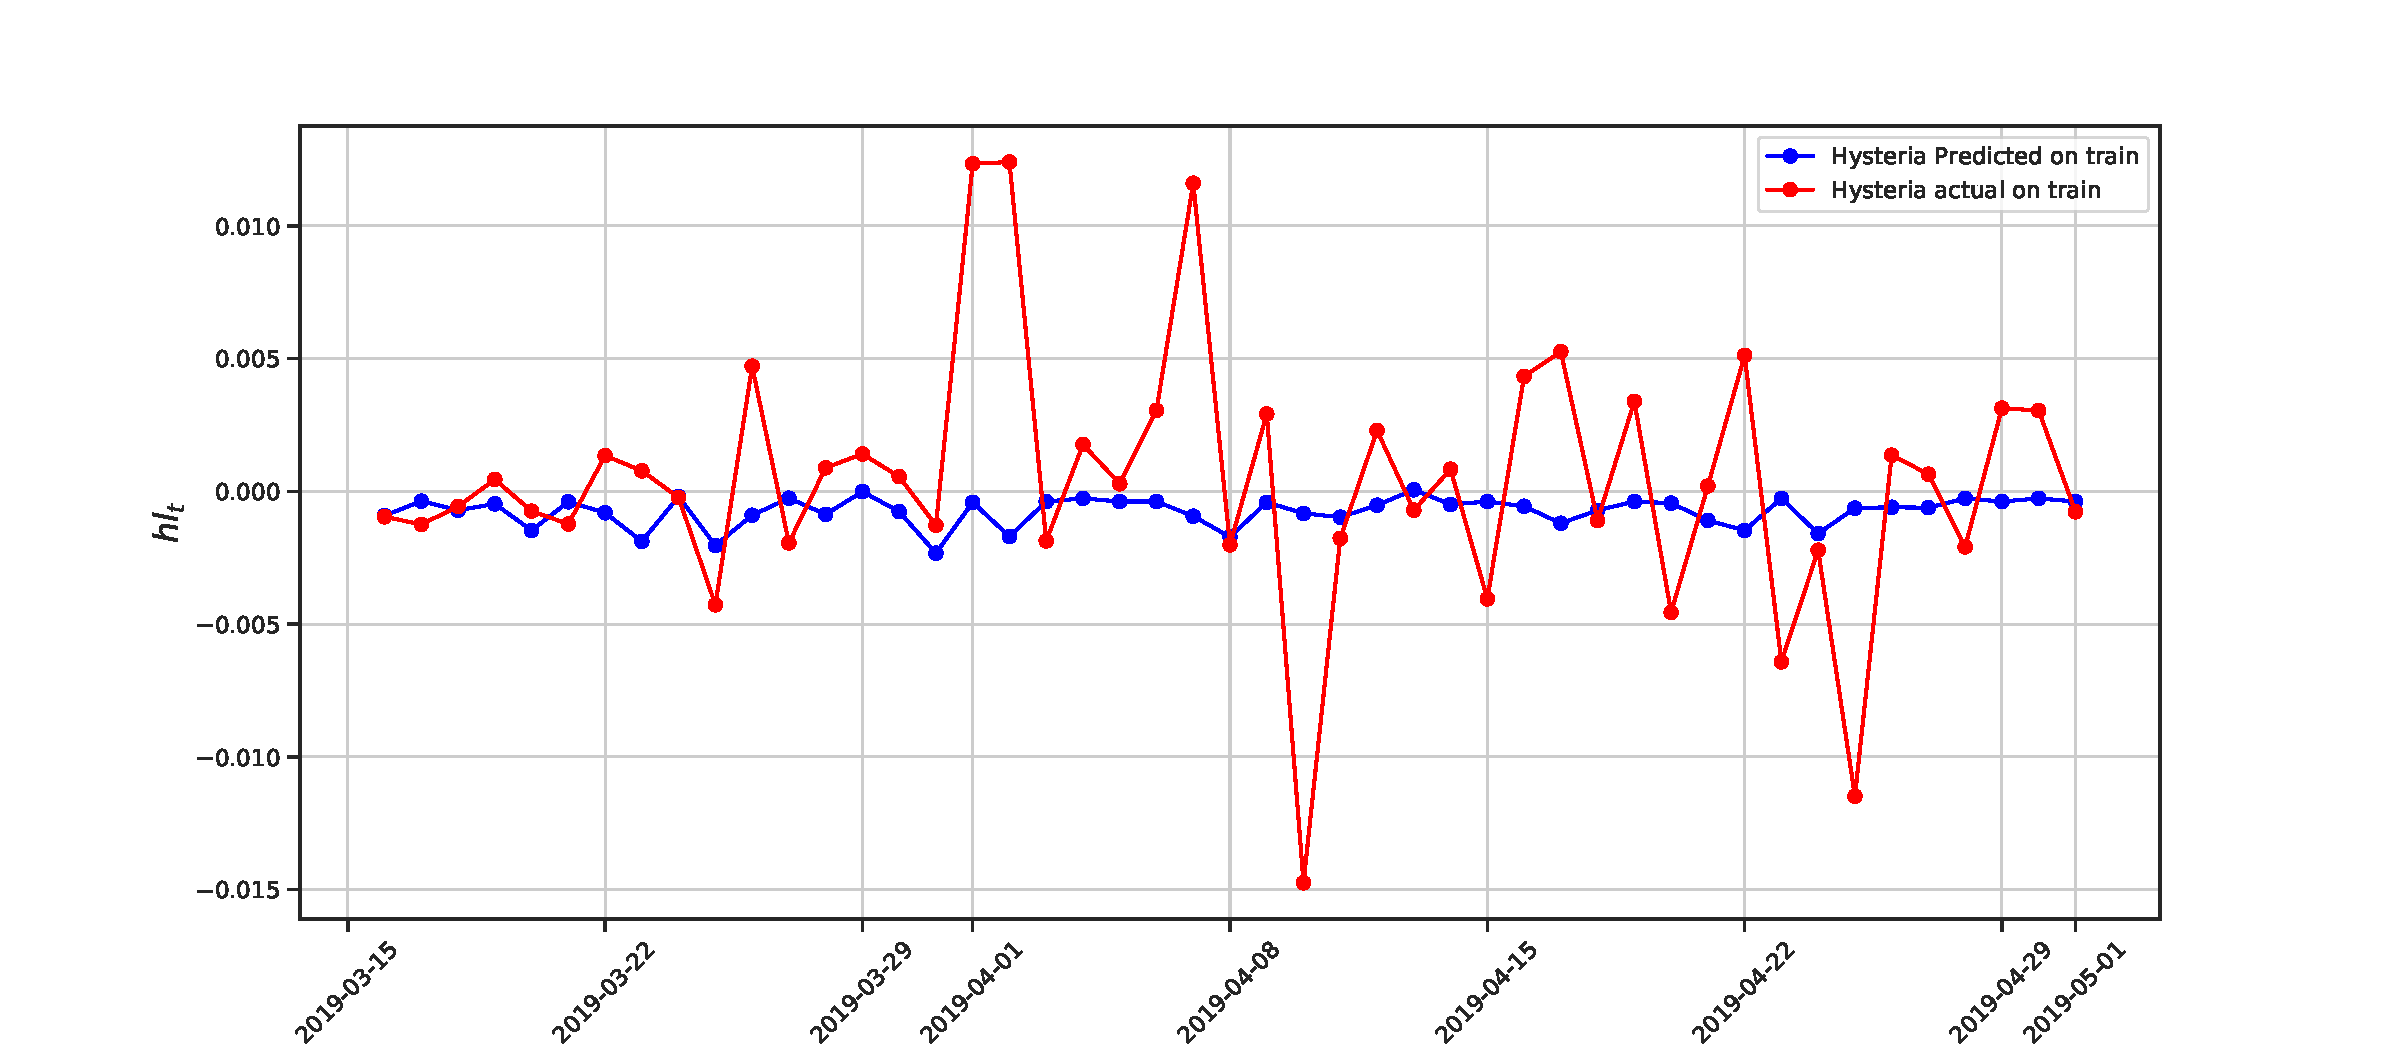
\includegraphics[width=0.9\textwidth]{notebooks/data/2019_hys_senti.pdf}
		\caption{$hl_{t}$  for 2019-03-16 to 2019-05-01 test set.}
		\label{fig:sent2019}
	\end{minipage}
\end{figure}




\subsection{Conclusion on Modeling the Ether price with social media}

The test $\%sMAPE$ on the price prediction for 2019  was $9.9\%$. The naive forecast scored $8.4\%$.


\section{Conclusions}



\begin{itemize}
	\item Unfortunately none of the implemented techniques were able to outperform the naive forecast. However, we still believe that through social media, the erratic behavior of the price can be predicted.
	\item We believe that the reason for the somewhat disappointing results for social media comes from the fact that the scoring systems of sentiment analysis were poorly designed. Techniques related to natural language processing should be implemented.
	\item Using Single layer perceptrons with enough processing power showed signs of being able to surpass the naive forecast.
\end{itemize}

\section{Comments on sections 4 and 5}
The deadline for this project was on 20 of may, I had to rush in this final part. As soon as I got some time, I will re do those sections.

% \begin{thebibliography}{1}
% \bibitem{1}
% Cleveland, W.S. (1979) “Robust Locally Weighted Regression and Smoothing Scatterplots”. Journal of the American Statistical Association 74 (368): 829-836.

% \bibitem{2}
% Oraintara, S., Chen, Y. J., \& Nguyen, T. Q. (2002). Integer fast Fourier transform. IEEE Transactions on Signal Processing, 50(3), 607-618.

% \end{thebibliography}

% ==============================================================================
% START: Methods, Results, Discussions, Conclusion
% ==============================================================================